\documentclass[11pt, twoside, pdftex]{article}

% This includes all the settings that we should use for the document
\newcommand{\PDFTitle}{\productNameMed{} Tutorial}
\newcommand{\commonPath}{../../Common}
\newcommand{\datePublished}{Mar 2022}

\newcommand{\versnum}{21.1} %version number quartus/AMP
\newcommand{\quartusname}{Quartus\textsuperscript{\textregistered} Prime}	
\newcommand{\textBar}{For \quartusname{} \versnum{}}
\newcommand{\thisyear}{2022 } %for copyright
\newcommand{\company}{FPGAcademy.org}
\newcommand{\longteamname}{FPGAcademy.org}
\newcommand{\teamname}{FPGAcademy}
\newcommand{\website}{FPGAcademy.org}

\newcommand{\productAcronym}{AMP}
\newcommand{\productNameShort}{Monitor Program}

\newcommand{\productNameMedTM}{Monitor Program}
\newcommand{\productNameMed}{Monitor Program}

%\newcommand{\headerLogoFilePath}[1]{#1/FPGAcademy.png}



\setlength\topmargin{-0.25in}
\setlength\headheight{0in}
\setlength\headsep{0.35in}
\setlength\textheight{8.5in}
\setlength\textwidth{7in}
\setlength\oddsidemargin{-0.25in}
\setlength\evensidemargin{-0.25in}
\setlength\parindent{0.25in}
\setlength\parskip{0in} 

\pdfpagewidth 8.5in
\pdfpageheight 11in

% listings is a package that supports encapsulating source code in LaTeX conveniently

\usepackage{listings}
% add support for graphics
\usepackage{graphicx}
\usepackage[usenames, dvipsnames]{color}

\def\expandparam\lstinputlisting[#1]#2{\edef\tmp{\noexpand\lstinputlisting[#1]{#2}}\tmp}

\widowpenalty 10000
\clubpenalty 10000

%%%%%%%%%%%%%%%%%%%% Source Code Formatting %%%%%%%%%%%%%%%%%%%%
\definecolor{globalCommentColour}{rgb}{0.588,0.588,0.588}

%%%%%%%%%%%%%%%%%%%%%%%%%%%%%%%%%%%%%%%%%%%%%%%%%%%%
% Defining a NiosII ASM highlighter for lstlisting
\lstdefinelanguage[NiosII]{Assembler} {
 	morekeywords={add, addi, and, andhi, andi, beq, bge, bgeu, bgt, bgtu, ble,  bleu, blt, bltu, bne, br, break,% 
 	bret, call, callr, cmpeq, cmpeqi, cmpge, cmpgei, cmpgeu, cmpgeui, cmpgt, cmpgti, cmpgtu, cmpgtui, cmple,%
 	cmplei, cmpleu, cmpleui, cmplt, cmplti, cmpltu, cmpltui, cmpne, cmpnei, custom, div, divu, eret, flushd,%
 	flushda, flushi, flushp, initd, initda, initi, jmp, jmpi, ldb, ldbio, ldbu, ldbuio, ldh, ldhio, ldhu, ldhuio,%
 	ldw, ldwio, mov, movhi, movi, movia, movui, mul, muli, mulxss, mulxsu, mulxuu, nextpc, nop, nor, or, orhi, ori,%
 	rdctl, rdprs, ret, rol, roli, ror, sll, slli, sra, srai, srl, srli, stb, stbio, sth, sthio, stw, stwio,%
 	sub, subi, sync, trap, wrctl, wrtcl, wrprs, xor, xori, xorhi, xori},% 	
 	morekeywords=[2]{.abort, .ABORT, .align, .app-file, .ascii, .asciz, .balign, .byte, .comm, .data, .def,%
 	.desc, .dim, .double, .eject, .else, .end, .endef, .endif, .equ, .equiv, .err, .extern, .file, .fill, .float,%
 	.global, .globl, .hword, .ident, .if, .include, .int, .irp, .irpc, .lcomm, .lflags, .line, .linkonce, .ln,%
 	.list, .long, .macro, .mri, .nolist, .octa, .org, .p2align, .psize, .quad, .rept, .sbttl, .scl, .section,%
 	.set, .short, .single, .size, .sleb128, .skip, .space, .stadb, .stabn, .stabs, .string, .symver, .tag,%
 	.text, .title, .type, .val, .uleb128, .word},% 	
 	morekeywords=[3]{et, bt, gp, sp, fp, ea, sstatus, ra, pc, status, estatus, bstatus, ienable, ipending, cpuid,%
 	exception, pteaddr, tlbacc, tlbmisc, eccinj, badaddr, config, mpubase, mpuacc},% 	
 	sensitive=t,%
 	alsoletter=.,%
	morestring=[b]",%
 	morecomment=[s]{/*}{*/},%
 	morecomment=[l]\#,%
   }[keywords,comments,strings]
   
   %% NOTE: morekeywords=[2] are GNU directives.
   
   \definecolor{niosInstructionColour}{rgb}{0.000,0.608,0.000}
   \definecolor{niosDirectiveColour}{rgb}{0.000,0.000,0.902}
   \definecolor{niosSpecialRegColour}{rgb}{0.000,0.000,0.000}
   \definecolor{niosStringColour}{rgb}{0.808,0.482,0.000}
   
   %% NOTE: To make bold use: =\bfseries\color{<colour>}
   \lstdefinestyle{defaultNiosStyle} {
   language=[NiosII]{Assembler},
   stringstyle=\color{niosStringColour},
   keywordstyle=\color{niosInstructionColour},
   keywordstyle=[2]\color{niosDirectiveColour},
   keywordstyle=[3]\itshape\color{niosSpecialRegColour}
   }
%%%%%%%%%%%%%%%%%%%%%%%%%%%%%%%%%%%%%%%%%%%%%%%%%%%%

%%%%%%%%%%%%%%%%%%%%%%%%%%%%%%%%%%%%%%%%%%%%%%%%%%%%
% Defining a ArmA9 ASM highlighter for lstlisting
\lstdefinelanguage[ArmA9]{Assembler} {
 	morekeywords={ADC, ADD, ADDS, AND, ANDS, B, BAL, BEQ, BGE, BGT, BL, BLT, BIC, BKPT, BLX, BNE, BX, CDP, CLZ, CMN, CMP, EOR,%
 	EORS, LDC, LDM, LDR, LDRB, LDRBT, LDRH, LDRSB, LDRSH, LDRT, LSL, MCR, MLA, MOV, MOVW, MOVT, MRC, MRS, MSR, MUL, MVN, ORR, PLD,%
 	ROR, RSB, RSC, SBC, SMLAL, SMULL, STC, STM, STR, STRB, STRBT, STRH, STRT, SUB, SUBS, SWI, SWP, SWPB, TEQ, UMLAL,
 	PUSH, POP, MOVS, RORS, LSR},%
 	morekeywords=[2]{.abort, .ABORT, .align, .app-file, .ascii, .asciz, .balign, .byte, .comm, .data, .def,%
 	.desc, .dim, .double, .eject, .else, .end, .endef, .endif, .equ, .equiv, .err, .extern, .file, .fill, .float,%
 	.global, .globl, .hword, .ident, .if, .include, .int, .irp, .irpc, .lcomm, .lflags, .line, .linkonce, .ln,%
 	.list, .long, .macro, .mri, .nolist, .octa, .org, .p2align, .psize, .quad, .rept, .sbttl, .scl, .section,%
 	.set, .short, .single, .size, .sleb128, .skip, .space, .stadb, .stabn, .stabs, .string, .symver, .tag,%
 	.text, .title, .type, .val, .vectors, .uleb128, .word},%
 	morekeywords=[3]{SP, PC, MIDR, CTR, TCMTR, TLBTR, MPIDR, ID_PFR0, ID_PFR1, ID_DFR0, ID_MMFR0, ID_MMFR1, ID_MMFR2,%
 	ID_MMFR3, ID_ISAR0, ID_ISAR1, ID_ISAR2, ID_ISAR3, ID_ISAR4, CCSIDR, CLIDR, AIDR, CSSELR, TTBR0, TTRB1, TTBR2, DACR,%
 	DFSR, IFSR, ADFSR, AIFSR, DFAAR, IFAR, ICIALLUIS, BPIALLIS, PAR, ICIALLU, ICIMVAU, BPIALL, DCIMVAC, DCISW, V2PCWPR,%
 	DCCVAC, DCCSW, DDIMVAC, DCISW, TLBALLIS, TLBIMVAIS, TLBIASIDIS, TLBIMVAAIS, TLBIALL, TLBIMVA, TLBIASID, TLBIMVAA,%
 	PMCR, PMCNTENSET, PMCNTENCLR, PMOVSR, PMSWINC, PMSELR, PMXEVTYPER, PMXEVCNTR, PMUSERENR, PMINTENSET, PMINTENCLR,%
 	PRRR, NRRR, PLEIDR, PLEASR, PLEFSR, PLEUAR, PLEPCR, VBAR, MVBAR, ISR, FCSEIDR, CONTEXTIDR, TPIDRURW, TPIDRURO, TPIDRPRW},%
 	sensitive=f,%
 	alsoletter=.,%
	morestring=[b]",%
 	morecomment=[s]{/*}{*/},%
 	morecomment=[l]{//},%
   }[keywords,comments,strings]
   
   %% NOTE: morekeywords=[2] are GNU directives.
   
   \definecolor{armInstructionColour}{rgb}{0.000,0.608,0.000}
   \definecolor{armDirectiveColour}{rgb}{0.000,0.000,0.902}
   \definecolor{armSpecialRegColour}{rgb}{0.000,0.000,0.000}
   \definecolor{armStringColour}{rgb}{0.808,0.482,0.000}
   
   \lstdefinestyle{defaultArmStyle} {
   language=[ArmA9]{Assembler},
   stringstyle=\color{armStringColour},
   keywordstyle=\color{armInstructionColour},
   keywordstyle=[2]\color{armDirectiveColour},
   keywordstyle=[3]\itshape\color{armSpecialRegColour}
   }
%%%%%%%%%%%%%%%%%%%%%%%%%%%%%%%%%%%%%%%%%%%%%%%%%%%%

%%%%%%%%%%%%%%%%%%%%%%%%%%%%%%%%%%%%%%%%%%%%%%%%%%%%
% Defining style for the verilog.

\definecolor{verilogCommentColour}{rgb}{0.000,0.502,0.000}

\lstdefinestyle{defaultVerilogStyle} {
language={Verilog},
keywordstyle=\color{blue},
commentstyle=\color{verilogCommentColour}
}
%%%%%%%%%%%%%%%%%%%%%%%%%%%%%%%%%%%%%%%%%%%%%%%%%%%%

%%%%%%%%%%%%%%%%%%%%%%%%%%%%%%%%%%%%%%%%%%%%%%%%%%%%
% Defining style for the vhdl.
\lstdefinestyle{defaultVHDLStyle} {
language={VHDL},
keywordstyle=\color{blue},
commentstyle=\color{verilogCommentColour}
}
%%%%%%%%%%%%%%%%%%%%%%%%%%%%%%%%%%%%%%%%%%%%%%%%%%%%

%%%%%%%%%%%%%%%%%%%%%%%%%%%%%%%%%%%%%%%%%%%%%%%%%%%%
% Java
\definecolor{javaStringColour}{rgb}{0.808,0.482,0}
%%%%%%%%%%%%%%%%%%%%%%%%%%%%%%%%%%%%%%%%%%%%%%%%%%%%

%%%%%%%%%%%%%%%%%%%%%%%%%%%%%%%%%%%%%%%%%%%%%%%%%%%%
% Defining language styles
% C
\definecolor{CStringColour}{rgb}{0.808,0.482,0}
%%%%%%%%%%%%%%%%%%%%%%%%%%%%%%%%%%%%%%%%%%%%%%%%%%%%

%%%%%%%%%%%%%%%%%%%%%%%%%%%%%%%%%%%%%%%%%%%%%%%%%%%%
% Defining extended LaTeX language.
\lstdefinelanguage[LocalLaTeX]{TeX}[LaTeX]{TeX}%
 	{moretexcs={bf, it, sf, lstset},%
   	}%

\lstdefinestyle{defaultLocalLatexStyle} {
language=[LocalLatex]{TeX},
keywordstyle=\color{blue}\bfseries,
keywordstyle=[2]\color{blue},
keywordstyle=[3]\color{blue}\bfseries
}
%%%%%%%%%%%%%%%%%%%%%%%%%%%%%%%%%%%%%%%%%%%%%%%%%%%%

\lstset{
%language = C,
%language = Verilog,
%basicstyle=\color{black}\rmfamily\ttfamily,
basicstyle=\small\color{black}\ttfamily,
commentstyle=\small\color{globalCommentColour}\itshape\ttfamily,
keywordstyle=\small\color{blue}\bfseries\ttfamily,
showstringspaces=false,
frame=none, %lines % boxed listings
breaklines=true,
breakatwhitespace=true,
tabsize=4
}
%%%%%%%%%%%%%%%%%%%%%%%%%%%%%%%%%%%%%%%%%%%%%%%%%%%%%%%%%%%%%%%%


%\usepackage[centering]{geometry}.
%%%%%%%%%%%%%%%%%%%%%%%%%%%%%%%%%%%%%%%%%%%%%%%%%%%
% Document Settings
\usepackage[labelsep=period]{caption}
% we can choose a better font later
%\usepackage{palatino}
\usepackage{fourier}
%\fontencoding{T1}
% include common used symbols
\usepackage{textcomp}
% add support for graphics
\usepackage{graphicx}
\usepackage[usenames, dvipsnames]{color}
% enable to draw thick or thin table hlines
\setlength{\doublerulesep}{\arrayrulewidth}
\usepackage{longtable}
\setlongtables
%\usepackage{array}
% It may be better to use PDFLaTeX as it can generate bookmarks for the
% document

% Add some useful packages
\usepackage{ae,aecompl}
\usepackage{epsfig,float,times}

% reset the font for section
\usepackage{sectsty}
%\allsectionsfont{\fontfamily{ptm}\selectfont}
\allsectionsfont{\usefont{OT1}{phv}{bc}{n}\selectfont}

% use compact space for sections
\usepackage[compact]{titlesec}
\titlespacing{\section}{0pt}{0.2in}{*0}
\titlespacing{\subsection}{0pt}{0.1in}{*0}
\titlespacing{\subsubsection}{0pt}{0.05in}{*0}

% fancyhdr header and footer customization
\usepackage{layout}
\usepackage{fancyhdr}
\pagestyle{fancy}
\fancyhead{}
\fancyhead[R]{\textit{\tiny{\textBar}}}
\fancyfoot{}
\fancyfoot[LO,
RE]{\textrm{\href{https://www.fpgacademy.org}{\small \longteamname}} \\ {\small \datePublished }}
\fancyfoot[RO, LE]{\small \thepage}
% two-side settings
%\fancyhead{} % clear all header fields
%\fancyfoot{} % clear all footer fields
%\fancyfoot[LE,RO]{\thepage}
\renewcommand{\headrulewidth}{2pt}
\renewcommand{\headrule}{{\color{blue} \hrule width\headwidth height\headrulewidth \vskip-\headrulewidth}}
\renewcommand{\footrulewidth}{0pt}

% Format the footer on page 1
\fancypagestyle{plain}{
\fancyhead{}
\fancyfoot{}
\fancyfoot[LO,
RE]{\textrm{\href{https://www.fpgacademy.org}{\small \longteamname}} \\ {\small \datePublished }}
\fancyfoot[RO, LE]{\small \thepage}
\renewcommand{\headrulewidth}{0pt}
}
% adjust some setting to try to make the figure stay in the same page with text
% Reference: 	http://www.cs.uu.nl/~piet/floats/node1.html
%   			http://mintaka.sdsu.edu/GF/bibliog/latex/floats.html
%   General parameters, for ALL pages:
\renewcommand{\topfraction}{0.9}	% max fraction of floats at top
\renewcommand{\bottomfraction}{0.8}	% max fraction of floats at bottom
%   Parameters for TEXT pages (not float pages):
\setcounter{topnumber}{3}
\setcounter{bottomnumber}{3}
\setcounter{totalnumber}{5}     % 2 may work better
\setcounter{dbltopnumber}{2}    % for 2-column pages
\renewcommand{\dbltopfraction}{0.9}	% fit big float above 2-col. text
\renewcommand{\textfraction}{0.07}	% allow minimal text w. figs
%   Parameters for FLOAT pages (not text pages):
\renewcommand{\floatpagefraction}{0.7}	% require fuller float pages
% N.B.: floatpagefraction MUST be less than topfraction !!
\renewcommand{\dblfloatpagefraction}{0.7}	% require fuller float pages
%%%%%%%%%%%%%%%%%%%%%%%%%%%%%%%%%%%%%%%%%%%%%%%%%%%
% remember to use [htp] or [htpb] for placement
%%%%%%%%%%%%%%%%%%%%%%%%%%%%%%%%%%%%%%%%%%%%%%%%%%%

% set no indent for paragraph
\setlength{\parindent}{0em}
\addtolength{\parskip}{11pt}
\newcommand{\compact}{[topsep=0pt]}
% use this package to reduce space
\usepackage{enumitem}
\usepackage{multirow}
\usepackage{rotating}
\usepackage{pifont}
\usepackage{dingbat}
\newcommand{\itemsecond}{$\circ$}
%
%%%%%%%%%%%%%%%%%%
\date{}
\author{}
%%%%%%%%%%%%%%%%%%
\newcommand{\de}{DE-series}
\newcommand{\up}{FPGAcademy}
\newcommand{\fabric}{Avalon Switch Fabric}
\newcommand{\TODO}[1]{\textcolor{red}{\textbf{TODO}: #1}}
\def\registered{{\ooalign{\hfil\raise .00ex\hbox{\scriptsize R}\hfil\crcr\mathhexbox20D}}}

% enable url and reference(bookmarks) in pdf
\usepackage{url}
\usepackage[pdftex, colorlinks]{hyperref}
\hypersetup{%
pdftitle={\PDFTitle},
linkcolor=blue,
hyperindex=true,
pdfauthor={\longteamname},
pdfkeywords={FPGAcademy, Academic Program, Example System},
bookmarksnumbered,
bookmarksopen=false,
filecolor=blue,
pdfstartview={FitH},
urlcolor=blue,
plainpages=false,
pdfpagelabels=true,
linkbordercolor={1 1 1} %no color for link border
}%
%%%%%%%%%%%%%%%%%%%%%%%%%%%%%%%%%%%%%%%%%%%%%%%%%%%
\setlength{\fboxsep}{0.7pt}
\setlength{\fboxrule}{0.5pt}

\newcommand{\red}[1]{{\color{red}\sf{#1}}}
\newcommand{\blue}[1]{{\color{blue}\sf{#1}}}



%%%%%%%%%%%%%%%%%%%%%%%%%
% Add title
\newcommand{\doctitle}{\productNameMed{} \\ Tutorial for Nios\textsuperscript{\textregistered} V}
\newcommand{\dochead}{\productNameMed{} Tutorial for Nios\textsuperscript{\textregistered} V}
% Usually no need to change these two lines
\title{\fontfamily{phv}\selectfont{\doctitle} }
\chead{ \small{\textsc{\bfseries \dochead} } }
% Customizations
%%%%%%%%%%%%%%%%%%%%%%%%%
% Allows multiple figures per page

\renewcommand\floatpagefraction{.9}
\renewcommand\topfraction{.9}
\renewcommand\bottomfraction{.9}
\renewcommand\textfraction{.1}   
\setcounter{totalnumber}{50}
\setcounter{topnumber}{50}
\setcounter{bottomnumber}{50}
\widowpenalty 10000
\clubpenalty 10000
\raggedbottom

%%%%%%%%%%%%%%%%%%
%%% DOCUMENT START
%\begin{document}
\begin{document}
\begin{table}
    \centering
    \begin{tabular}{p{5cm}p{4cm}}
        \hspace{-3cm}
        &
        \raisebox{1\height}{\parbox[h]{0.5\textwidth}{\Large\fontfamily{phv}\selectfont{\textsf{\doctitle}}}}
    \end{tabular}
    \label{tab:logo}
\end{table}

\colorbox[rgb]{0,0.384,0.816}{\parbox[h]{\textwidth}{\color{white}\textsf{\textit{\textBar}}}}

\thispagestyle{plain}
 
\section{Introduction}

This tutorial presents an introduction to the \productNameMed{}, 
which can be used to compile, assemble, download and
debug programs for the Intel Nios\textsuperscript{\textregistered}~V processor. 
In this tutorial we assume that the Nios V processor is being used as part of the DE1-SoC
Computer system. If a different hardware system is being used, then some parts of this 
tutorial may need to be modified accordingly.

The Monitor Program is a software application which runs on a
host PC, and communicates with a Nios~II hardware system on an
FPGA board. It can be used to compile/assemble a
Nios II software application, download the application onto the
FPGA board, and then debug the running application.   
It provides features that allow a user to:

\begin{itemize}
    \item Set up a Nios II project that specifies a desired
hardware system and software program
    \item Download the hardware system onto an FPGA board
    \item Compile software programs, specified in assembly language or C, and download the resulting machine code into the
hardware system
    \item Display the Nios~II machine code stored in memory
    \item Run the Nios~II processor, either continuously or by single-stepping instructions
    \item Examine and modify the contents of processor registers
    \item Examine and modify the contents of memory, as well as
memory-mapped registers in I/O devices
    \item Set breakpoints that stop the execution of a program at
a specified address, or when certain conditions are met
    \item Develop Nios~II programs that make use of device driver
functions provided through Intel's Hardware Abstraction Layer
(HAL)
\end{itemize}

The process of downloading and debugging a Nios~II program
requires an FPGA board to implement the Nios~II hardware system.
In this tutorial it is assumed that the reader has access to the
Intel DE1-SoC Development and Education board, connected to a
computer that has Quartus Prime 
and Nios~II Embedded Design Suite (EDS) software installed. Although a reader who does not have access to an FPGA board will
not be able to execute the Monitor Program commands described in
the tutorial, it should still be possible to follow the
discussion.


\subsection{Who should use the Monitor Program}

The Monitor Program is intended to be used in an educational
environment by professors and students. It is not intended for
commercial use.

\section{Installing the Monitor Program}

The Monitor Program is released as part of the University
Program Design Suite (UPDS). Before the UPDS can be installed on
a computer, it is necessary to first install Intel's Quartus\textsuperscript{\textregistered} Prime
CAD software (either the Lite, Standard, or Pro edition) 
and the Nios~II Embedded Design Suite (EDS). A particular release
of the Monitor Program can be used only with a corresponding version of the Quartus Prime software and Nios~II EDS. This software
can be obtained from the on Intel's website.

Once the Quartus Prime software and Nios~II EDS are installed, the UPDS can be installed.

Note that if the Quartus Prime software is re-installed at some
future time, then it will be necessary to re-install the Monitor
Program at that time.

\subsection{Using a Windows Operating System}

When using a Windows operating system, perform the following: 

\begin{enumerate}

\item Install the Monitor Program software (and related design files) by downloading the 
installation package from the 
\href{https://www.fpgacademy.org/tools.html}{FPGAcademy} website.
Specify the installed version of Quartus Prime software.
Then click on the {\it EXE} item in the displayed table, 
which links to an installation program called 
{\it intel\_fpga\_upds\_setup.exe}. When prompted to 
{\sf Run} or {\sf Save} this file, select {\sf Run}.
		  
\item The first screen of the installer is shown in Figure~\ref{fig:1}.
Click on the {\sf Next} button.

 \item The installer will display the License Agreement; if you accept the terms of this agreement, then click {\sf I Agree} to
continue.
	
\item The installer now displays the root directory where the
{\teamname} Design Suite will be installed.  
Click {\sf Next}.

\item The next screen, shown in Figure~\ref{fig:2}, lists the components that will be installed, which include the Monitor Program
software and University Program IP Cores. These IP Cores provide
a number of I/O device circuits that can be used in hardware
systems to be implemented on the FPGA board.

\item The installer is now ready to begin copying files. 
Click {\sf Install} to proceed and then click {\sf Next} after
the installation has been completed. 
If you answered {\sf Yes} when prompted about placing a shortcut on your Windows Desktop, then an icon 
\hbox{
\includegraphics[scale=0.65]{images/img_shortcut_sm.png}}
is provided on the Desktop that can be used to start the Monitor
Program.

\begin{figure}[H]
   	\begin{center}
           
\includegraphics[scale=0.7]{screenshots/figure1.png}
   	\end{center}
      \caption{Intel UPDS Setup Program.}
			\label{fig:1}
\end{figure}

\begin{figure}[H]
   	\begin{center}
            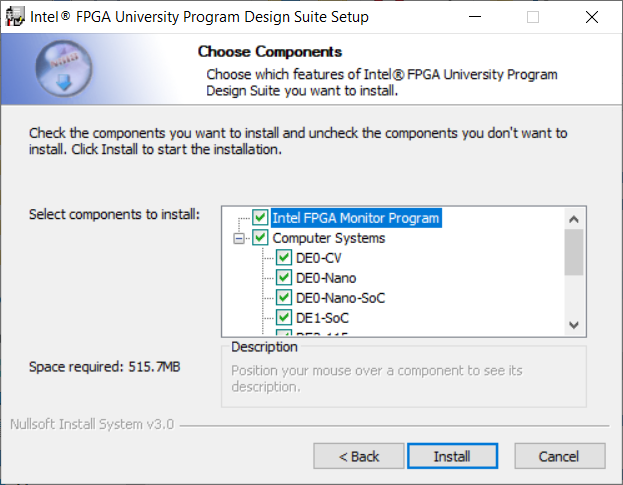
\includegraphics[scale=0.7]{screenshots/figure2.png}
   	\end{center}
      \caption{The components that will be installed.}
			\label{fig:2}
\end{figure}
~\\
	 
\item Now, the \teamname~ Design Suite is successfully installed on your computer, so click {\sf Finish} to
finish the installation.

\item Should an error occur during the installation procedure, a pop-up window will suggest the appropriate action. 
Possible errors include:
\begin{itemize}
\item Quartus Prime software is not installed or the Quartus Prime version is incorrect.
\item Nios~II EDS software is not installed or the version is incorrect.
\end{itemize}
\end{enumerate}

\subsection{Using a Linux* Operating System}

When using a Linux* operating system, perform the following:

\begin{enumerate} 
\item Install the Monitor Program software (and related design files) by downloading the 
installation package from the 
\href{https://www.fpgacademy.org/tools.html}{FPGAcademy} website.
Specify the installed version of Quartus Prime software.
Then click on the {\it TAR} item in the displayed table, 
which links to an installation tarball called 
{\it altera\_upds\_setup.tar}. 
Save this file to a directory of your choosing.

\item Using a console, navigate to the directory to which the
file was saved. Extract the contents of 
{\it intel\_fpga\_upds\_setup.tar} using the following command: 
{\bf tar -xf intel\_fpga\_upds\_setup.tar}.

\item Among the extracted files is a shell script named
{\it install\_intel\_fpga\_upds} which will be used to install the
UPDS. Ensure that the script is executable by using the following
command: {\bf chmod +x install\_intel\_fpga\_upds}. 

\item Run the installation script with superuser privileges by
using the following command: 
{\bf sudo ./install\_intel\_fpga\_upds}.

\item Follow the instructions displayed by the script to complete
the installation.

\end{enumerate}

\section{Main Features of the Monitor Program}

Each Nios II software application that is developed with the
\productNameMed{} is called a {\it project}. 
The Monitor Program works on one project at a time and keeps all information for that project in a single directory in the file
system. The first step is to create a directory to hold the project's files. To store the design files for this tutorial, 
we will use a directory named {\it Monitor\_Tutorial}. 
The running example for this tutorial is a simple 
assembly-language program that controls some lights on a 
DE1-SoC board.

If you are using a Windows* operating system, then
start the Monitor Program software either by double-clicking its
icon on the Windows Desktop or by accessing the program in the
{\sf Windows Start} menu under 
{\sf Intel > University Program > \productNameMed{}}. 
You should see a display similar to the one in Figure~\ref{fig:3}.

If you are using a Linux operating system, then
start the Monitor Program software by running the
{\it altera-monitor-program} shell script located in
{\it <path to Intel software>/University Program/Monitor Program/bin}.
You should see a display similar to the one in Figure~\ref{fig:3}.

\begin{figure}[H]
   \begin{center}
      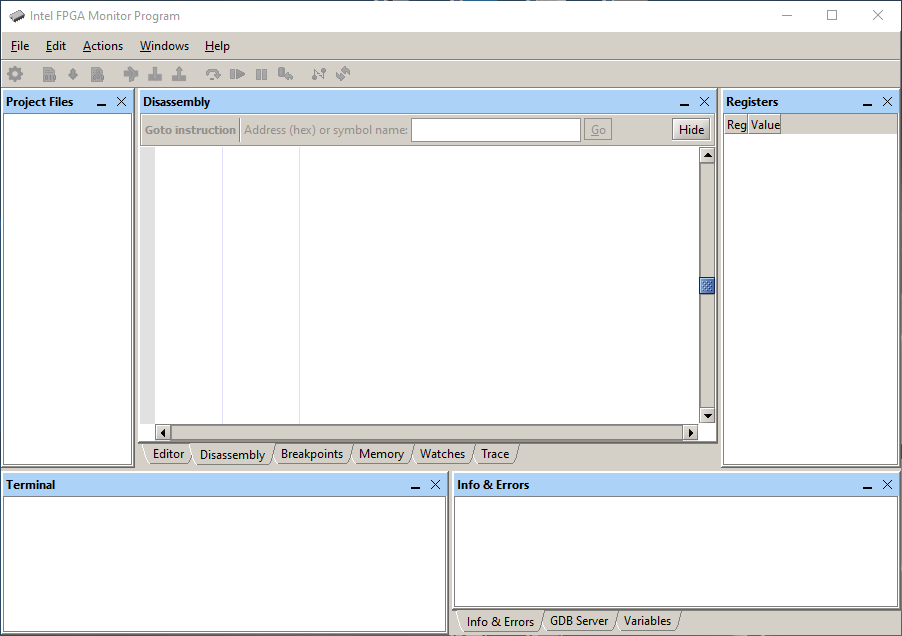
\includegraphics[scale=0.6]{screenshots/figure3.png}
   \end{center}
   \caption{The main Monitor Program display.} 
	\label{fig:3}
\end{figure}

This display consists of several windows that provide access to all of the features of the Monitor Program, which the user
selects with the computer mouse. Most of the commands 
provided by the Monitor Program can be accessed by using a set of
menus that are located below the title bar. For example, in
Figure~\ref{fig:3} clicking the left mouse button on
the {\sf File} command opens the menu shown in 
Figure~\ref{fig:4}. Clicking the left mouse 
button on the entry {\sf Exit} exits from the Monitor Program.  In most cases, whenever the mouse is used to select something,
the left button is used. Hence we will not normally specify which 
button to press. 

\begin{figure}[H]
   \begin{center}
      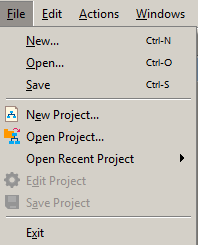
\includegraphics[scale=1]{screenshots/figure4.png}
   \end{center}
   \caption{An example of the {\sf File} menu.}
	 \label{fig:4}
	
\end{figure}

For some commands it is necessary to access two or more menus in
sequence. We use the convention {\sf Menu1 > Menu2 > Item} to
indicate that to select the desired command 
the user should first click the mouse button on {\sf Menu1}, 
then within this menu click on {\sf Menu2}, and then 
within {\sf Menu2} click on {\sf Item}. For example, 
{\sf File > Exit} uses the mouse to exit from the Monitor
Program. Many commands can alternatively be invoked 
by clicking on an icon displayed in the Monitor Program window. To see the command associated with an icon, position the mouse
over the icon and a tooltip will appear that displays 
the command name.

It is possible to modify the organization of the Monitor Program
display in Figure~\ref{fig:3} in many ways. 
Section 9 shows how to move, resize, close, and open windows
within the Monitor Program display.


\subsection{Creating a Project}
\label{sec:new_project}

To start working on a Nios II software application we first have
to create a new project, as follows: 
\begin{enumerate}
\item
Select {\sf File > New Project} to open the
{\it New Project Wizard}, which leads to the screen 
in Figure~\ref{fig:5}. The Wizard presents a sequence of screens for
defining a new project. Each screen includes a number of dialogs, as well as a message area at the bottom of the window.  
The message area is used to display error and information messages associated with the dialogs in the window. 
Double-clicking the mouse on an error message moves the cursor
into the dialog box that contains the source of the error.

\begin{figure}[H]
   \begin{center}
      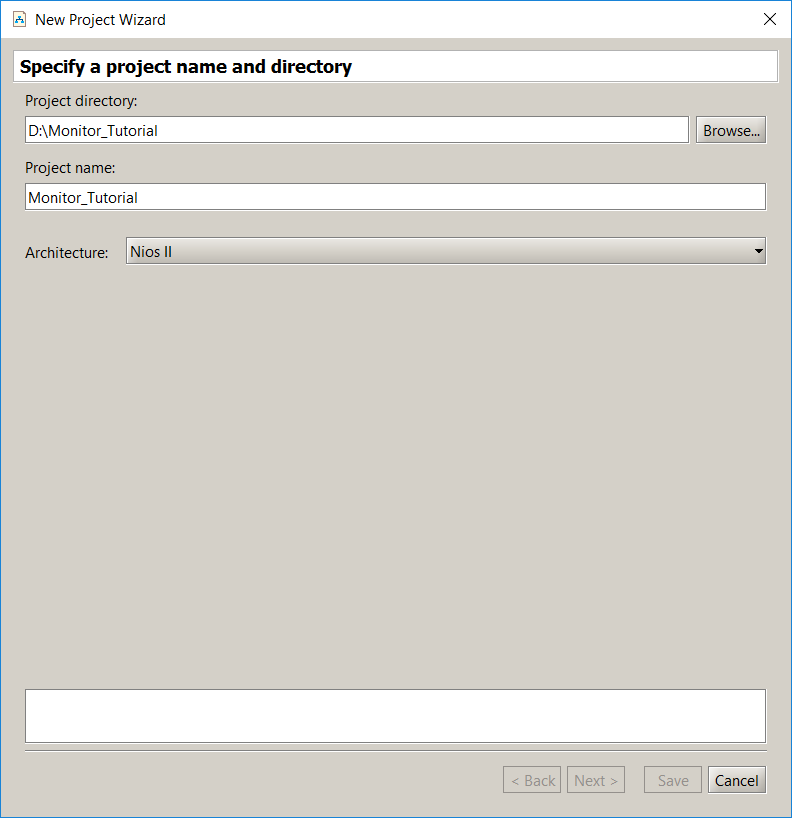
\includegraphics[scale=0.5]{screenshots/figure5.png}
   \end{center}
   \caption{Specifying the project directory and name.} 
	 \label{fig:5}
\end{figure}

In Figure~\ref{fig:5} we have specified the file system directory
{\it D:$\backslash$Monitor\_Tutorial} and the project 
name {\it Monitor\_Tutorial}. 
For simplicity, we have used a project name that matches the
directory name, but this is not required.

If the file system directory specified for the project does not
already exist, a message will be displayed indicating that this
new directory will be created. To select an existing directory
by browsing through the file system, click on the {\sf Browse} button. Note that a given directory may contain at most one
project.

The Monitor Program can be used with either an ARM* based system
or a Nios II-based system. The choice of a processor is made in
the window in Figure~\ref{fig:5} in the box labeled Architecture. 
We have chosen the Nios II architecture for this tutorial. 

\item
Click {\sf Next} to advance to the window shown in Figure~\ref{fig:6},
which is used to specify a particular system.
A hardware system to be implemented on the FPGA board is usually
generated by using Quartus's Platform Designer tool.
Information about creating systems using Platform Designer can be found in the \emph{Introduction to the Intel Platform Designer Tool} tutorial, 
which is available in the University Program section of Intel's website.

A system designed and generated by using Quartus Prime and its Platform Designer
tool is described in \emph{SOPCInfo} and \emph{SOF} files. The
former gives a high-level description of the system. 
The latter represents the FPGA
circuit that implements the designed system; this file can be downloaded into the FPGA chip on the board that is being used.   

Any system which contains a {\it Hard Processor System} (HPS) component must also specify the preloader to be run immediately following the circuit being downloaded. This preloader is used to configure the components within the HPS with the setting required for the specific board. 

The drop-down list on the {\sf Select a system} pane can be used
to choose the system to be used in the project. 
The Monitor Program includes a number of prebuilt computer
systems for Intel's Development and Education boards.
Since in this tutorial we assume that the user has access to a
DE1-SoC board, we will use a system called the DE1-SoC Computer. 
This computer includes a number of interfaces to 
input/output devices implemented in the FPGA fabric of the chip.
It was created using Quartus Prime and its Platform Designer tool.
It is represented by \emph{.sopcinfo} and \emph{.sof} files
which are automatically included when this computer is selected.
The DE1-SoC preloader is also automatically selected.

The user may also design and implement a custom system.
If the custom system is selected, then the user must manually 
specify the \emph{.sopcinfo} and \emph{.sof} files that define
the required system in the {\sf System details} pane. If the custom system contains an HPS, the user must select their board from the preloader dropdown menu.

In the top right corner of Figure~\ref{fig:6} there is a 
{\sf Documentation} button. 
Clicking on this button opens a user guide that provides all
information needed for developing Nios II programs for the
DE1-SoC Computer, such as the memory map for addressing all of
the I/O devices in the system. This file can also be accessed at
a later time by using the command 
{\sf Settings > System Settings} and then
clicking on the {\sf Documentation} button.

\begin{figure}[H]
   \begin{center}
      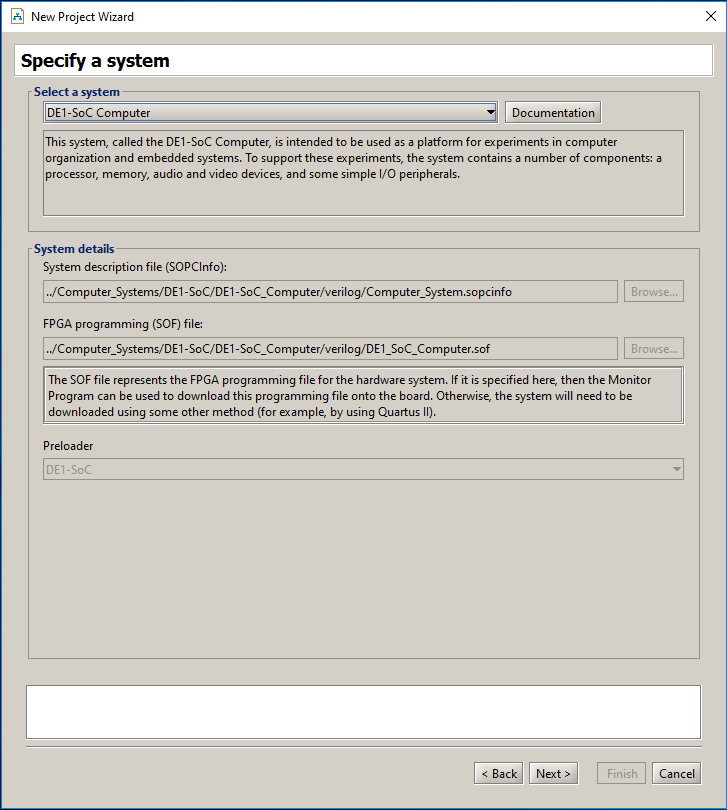
\includegraphics[scale=0.5]{screenshots/figure6.png}
   \end{center}
   \caption{Specifying the desired hardware system.} 
	 \label{fig:6}
\end{figure}

\item
Click {\sf Next} to advance to the screen in Figure~\ref{fig:7},
which is used to specify the program source files that are associated with the project.
The {\sf Program Type} drop-down list can be used to select one of the following program types:

\begin{itemize}
\item {\sf Assembly Program}: allows the Monitor Program to be
used with Nios II assembly-language code
\item {\sf C Program}: allows the Monitor Program to be used with
C code
\item {\sf Program with Device Driver Support}: this is an
advanced option, which can be used to develop programs that make
use of device driver software for the I/O devices in the Nios~II
hardware system.  Programs that use this option can be written in
either assembly, C, or C++ language (or any combination). 
More information about writing programs that use device drivers
can be found in Appendix B.
\item {\sf ELF or SREC File}: allows the Monitor Program to be
used with a precompiled program, in ELF or SREC format
\item {\sf No Program}: allows the Monitor Program to connect to
the Nios~II hardware system without first loading a program;
this can be useful if one wants to examine the current state of
some I/O devices without running an actual program.
\end{itemize}

\begin{figure}[H]
   \begin{center}
      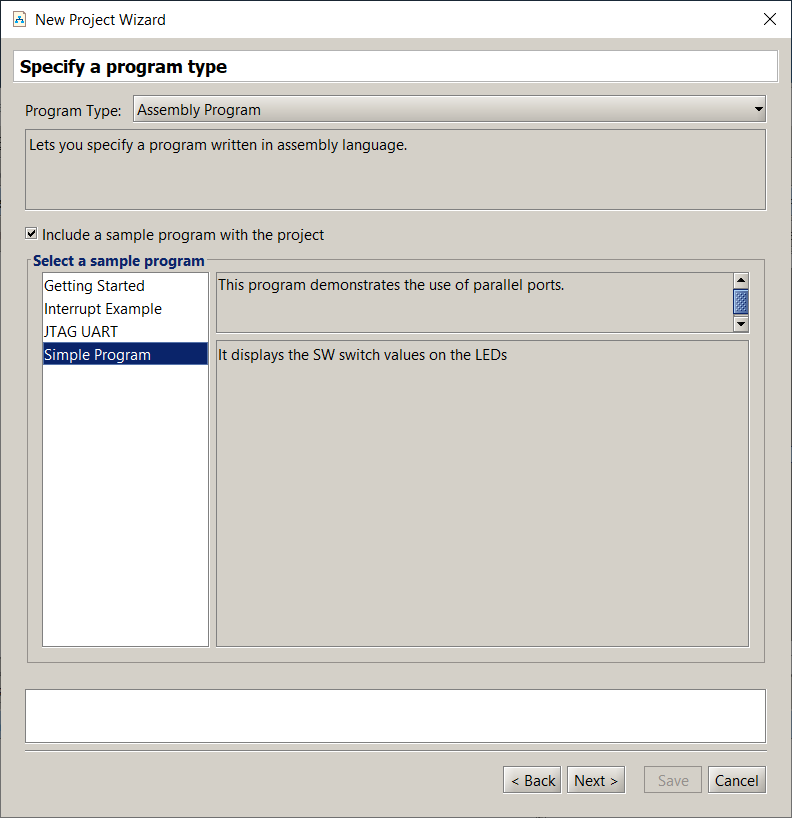
\includegraphics[scale=0.6]{screenshots/figure7.png}
   \end{center}
   \caption{Selecting a program type and sample program.} 
	 \label{fig:7}
\end{figure}


For our example, set the program type to {\sf Assembly Program}.
When the DE1-SoC computer has been selected for the project, 
it is possible to click on the
selection {\sf Include a sample program with the project}.

As illustrated in Figure~\ref{fig:7}, several sample 
assembly-language programs are available for this prebuilt
computer.  For our tutorial select the program named 
{\it Simple Program}. This is a very simple program which
continuously reads the state of the slider switches on the
DE1-SoC board and displays their state on the red LEDs.
The source code for the program is:

\lstset{style=defaultNiosStyle}
\begin{center}
\begin{minipage}[t]{16 cm}
\begin{lstlisting}
.text
.equ	LEDs, 0xFF200000
.equ	SWITCHES, 0xFF200040
.global _start
_start:
		movia	r2, LEDs			/* Address of red LEDs. */ 
		movia	r3, SWITCHES		/* Address of switches. */
LOOP:	ldwio 	r4, (r3)			/* Read the state of switches. */
		stwio	r4, (r2)			/* Display the state on LEDs. */
		br		LOOP
.end
\end{lstlisting}
\end{minipage}
\end{center}

Click {\sf Next} to advance to the screen in Figure~\ref{fig:8}.\\

\begin{figure}[H]
   \begin{center} 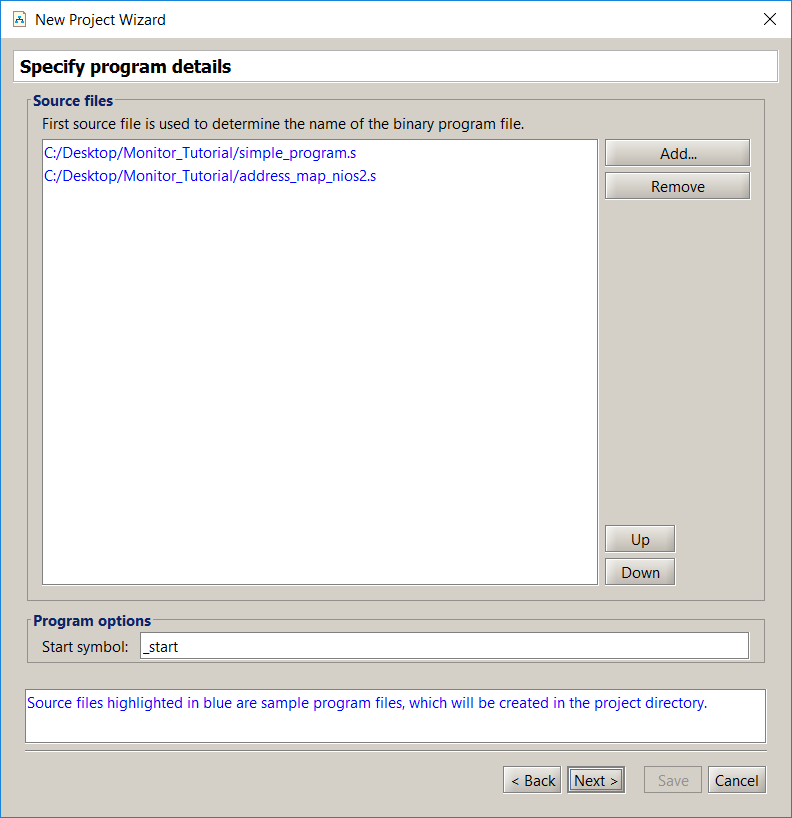
\includegraphics[scale=0.5]{screenshots/figure8.png}
   \end{center}
   \caption{Specifying source code files.} 
	 \label{fig:8}
\end{figure}

When a sample program has been
selected, the source code file(s) associated with this program
is listed in the {\sf Source files} box.  In this case, the source file is named {\it simple\_program.s}; this
file will be copied into the directory used for the project by
the Monitor Program. 
If a sample program is not used, then it is necessary to click
the {\sf Add} button and browse to select the desired source 
file(s).

Figure~\ref{fig:8} shows how it is possible to specify a label
that identifies the first instruction to be executed. 
In the {\it simple\_program.s} file, this label is called 
{\it \_start}, as indicated in the figure.

\item 
Click {\sf Next} to advance to the window in Figure~\ref{fig:9}.
This window is used to specify the connection to the FPGA board, the processor that should be used (some hardware systems may
contain multiple processors), and the terminal device.
The {\sf Host connection} drop-down list contains the physical
connection links (such as cables) that exist between the host computer and any FPGA boards connected to it. 
The processors available in the system are found in the 
{\sf Processor} drop-down list, and all 
terminal devices connected to the selected processor are displayed in the {\sf Terminal device} drop-down list. 
We discuss terminal devices in Section 6.

Accept the default choices that are displayed in Figure~\ref{fig:9}. If the Host Connection box is blank, make sure that 
the DE1-SoC board is connected to the host by a USB cable and
that its power is turned on. Then, press the {\sf Refresh} button and select the USB Blaster as the desired choice.
For the DE1-SoC board the required choice is DE-SoC.

\begin{figure}[H]
   \begin{center}
      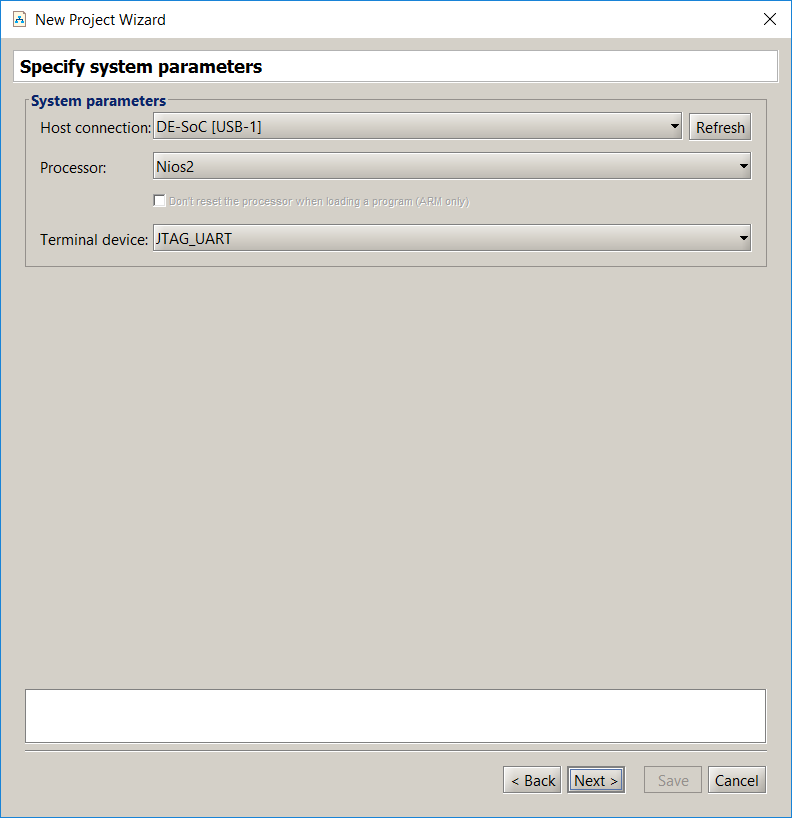
\includegraphics[scale=0.5]{screenshots/figure9.png}
   \end{center}
   \caption{Specifying system settings.} 
	 \label{fig:9}
\end{figure}

\item 
Click {\sf Next} to reach the final screen for creating the new
project, shown in Figure~\ref{fig:10}. This screen is used to specify memory settings that are needed for compiling and linking the
program.

\begin{figure}[H]
   \begin{center}
      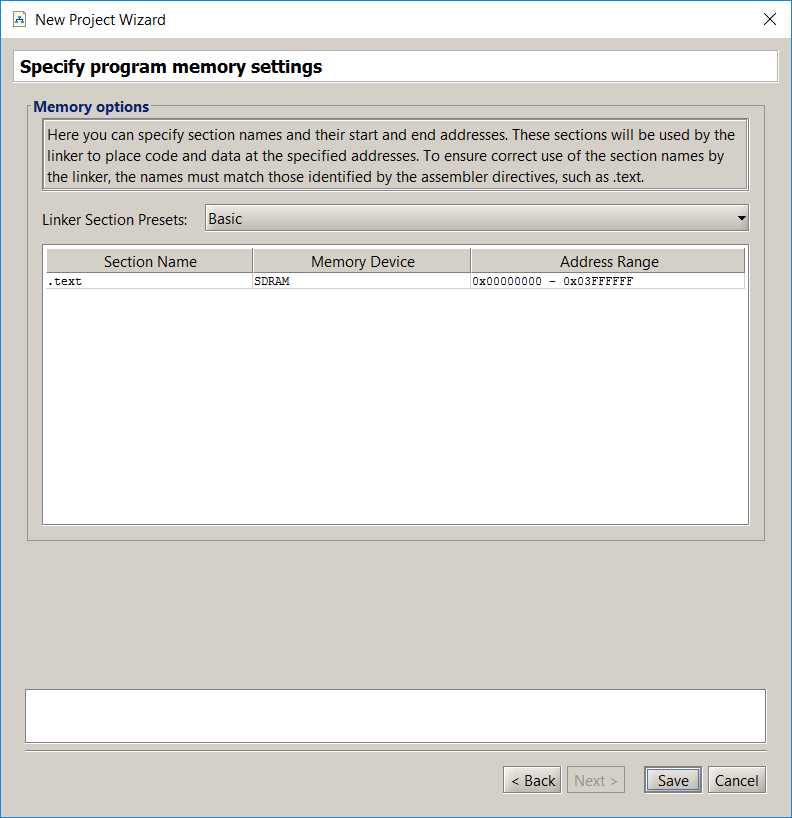
\includegraphics[scale=0.5]{screenshots/figure10.png}
   \end{center}
   \caption{Specifying memory settings.} 
	 \label{fig:10}
\end{figure}

There are two modes that can be selected. In the {\sf Basic}
mode, which does not provide explicitly for the use of
interrupts, the application program starts at memory address
0x00000000 as shown in the figure. A more general alternative
is to use the {\sf Interrupts} mode, which is discussed in
Section 8.  
The program in the {\it .text} section can start 
at some other address, as may be specified by the user.
To change the address, double-click on the {\it .text} entry
and change the address in the pop-up box that appears.

Click {\sf Finish} to complete the creation of the new project.  At this point, the Monitor Program displays the prompt shown in
Figure~\ref{fig:11}. Clicking {\sf Yes} instructs the Monitor Program to
download the hardware system associated with the project onto 
the FPGA board. It is also possible to download the system 
at a later time by using the Monitor Program command
{\sf Actions > Download System}. 
If the downloaded system contains more than one processor,
the Monitor Program will prompt you to halt the processors other
than the one being used for the current project. It is generally
recommended to halt the other processors because they can execute
without you knowing, resulting in unexpected behavior.

\begin{figure}[H]
   \begin{center}
      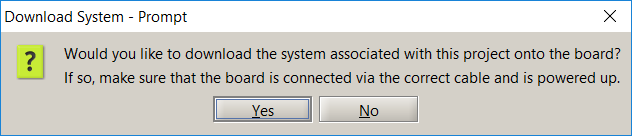
\includegraphics[scale=1]{screenshots/figure11.png}
   \end{center}
   \caption{Download the hardware system.} 
	 \label{fig:11}
\end{figure}

\subsubsection{Downloading a Nios~II Hardware System}

When downloading a Nios~II hardware system onto an FPGA board, 
it is important to consider the type of license that is included
in the hardware system for the processor.
The Nios~II processor uses a licensing scheme that provides two
modes of operation: 1. an evaluation mode that allows the
processor to be used with some restrictions when no
license is present, and 2. a normal mode that allows unrestricted
use when a license is present. Nios~II licenses can be purchased
from Intel, and are also available on a donated basis through
the University Program.  The prebuilt computer systems provided
with the Monitor Program, such as the DE1-SoC Computer, include a
Nios~II processor that has a license. However, if other systems
are being used with the Monitor Program, then it is
possible that a license is not present, and the Nios~II processor
may be used in the evaluation mode. In this case it is necessary
to use a different scheme, which is described in Section 5,
to download the Nios~II hardware system onto the FPGA board and activate the evaluation mode.

\end{enumerate}
%%%%%%%%%%%%%%%%%%%%%%%%%%%%%%%%%%%%%
%%% Compiling and Loading the Program
\subsection{Compiling and Loading the Program}

After successfully creating a project, its software files can be compiled/assembled and downloaded onto the FPGA board using the
following commands:

\begin{itemize}
\item \textsf{Actions > Compile} menu item or 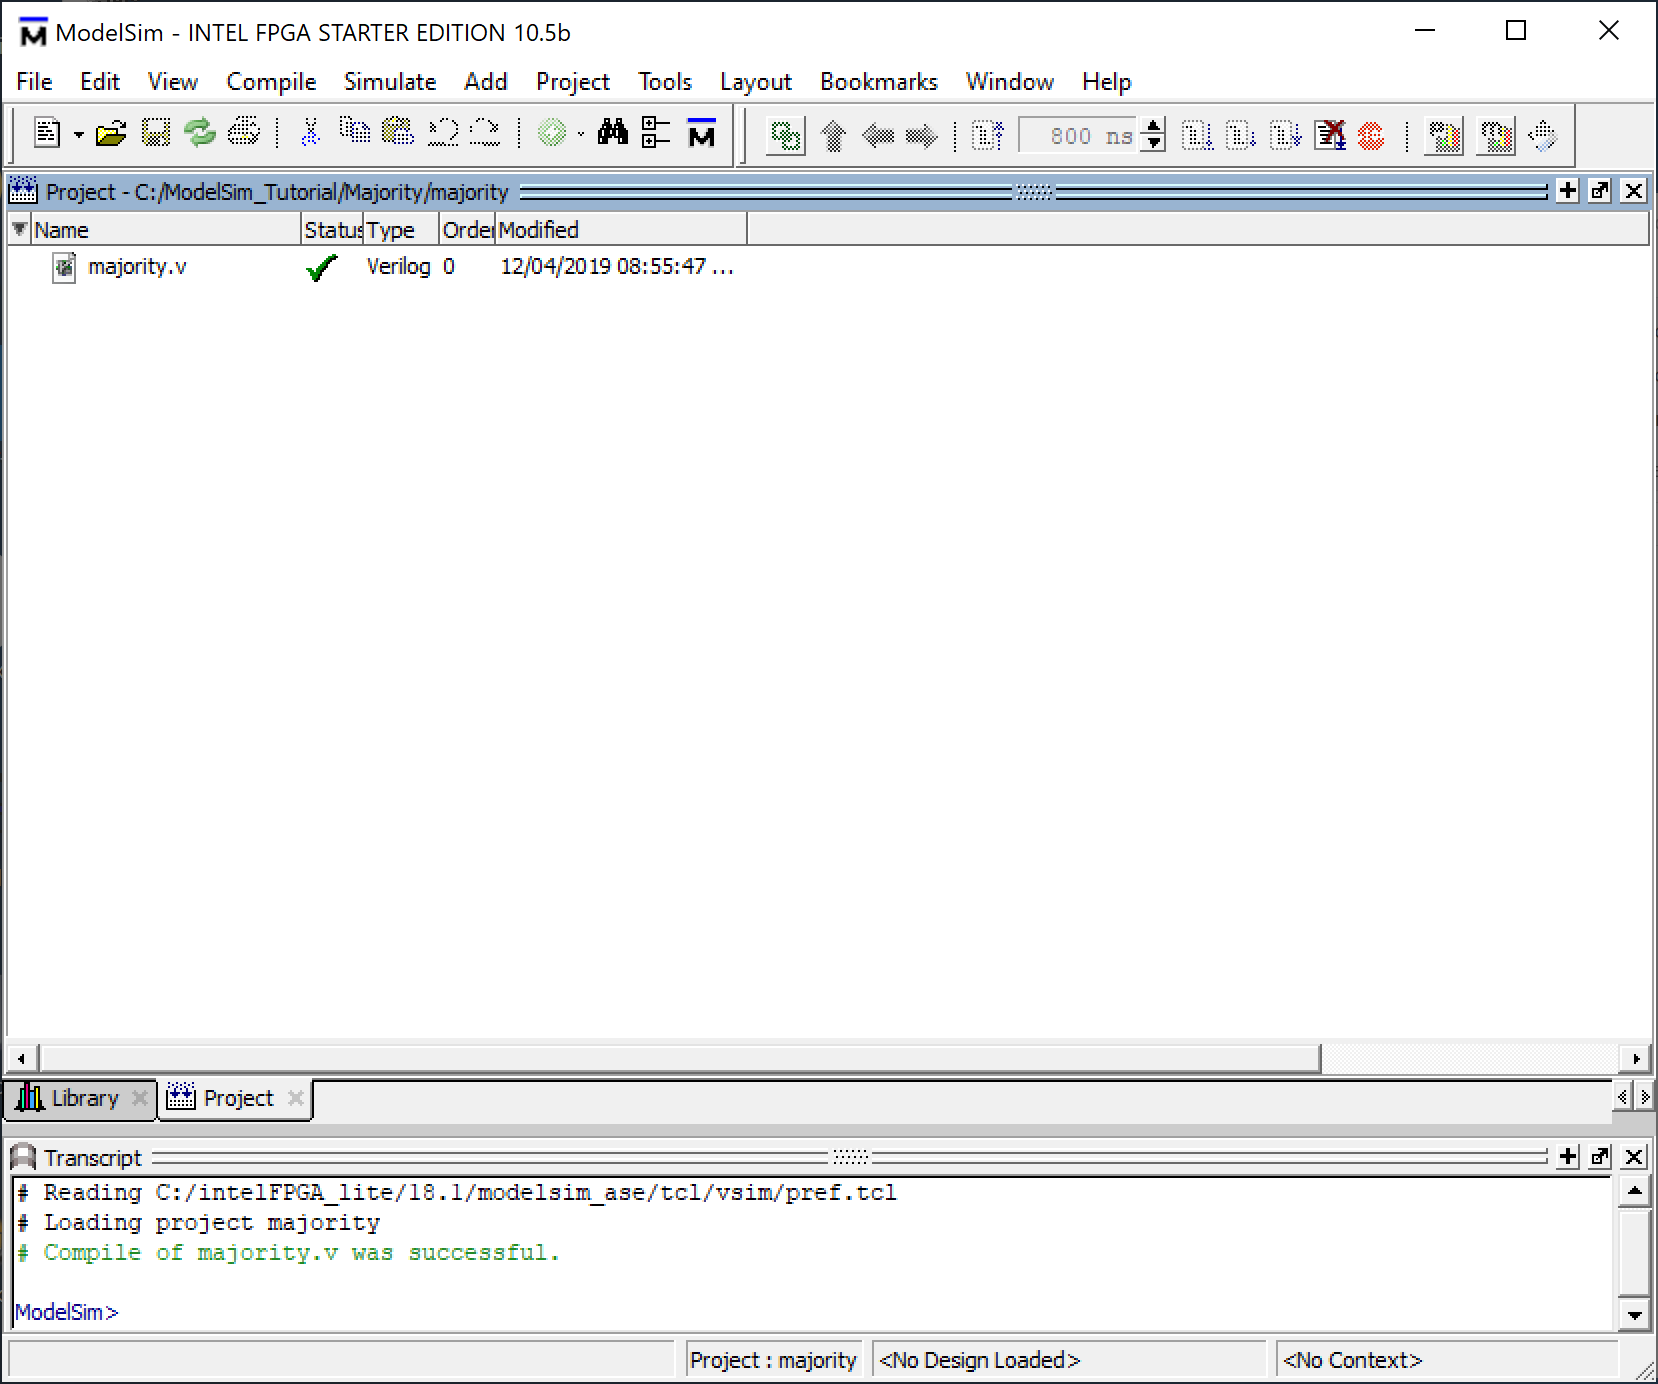
\includegraphics{toolbar/compile.png} 
icon: compiles the source files into an ELF and SREC file. Build
warnings and errors will show up in the 
\textsf{Info \& Errors} window.
The generated ELF and SREC files are placed in the project's directory.

\item \textsf{Actions > Load} menu item or 
\includegraphics{toolbar/load.png} icon:
loads the compiled SREC file onto the board and begins a
debugging session in the Monitor Program. Loading progress
messages are displayed in the \textsf{Info \& Errors} window.

\item \textsf{Actions > Compile~\&~Load} menu item or 
\includegraphics{toolbar/compile_load.png}
icon: performs the operations of both compilation and loading.
\end{itemize}

Our example project has not yet been compiled, so it cannot be
loaded (the \textsf{Load} option is disabled).  
Select the \textsf{Actions > Compile~\&~Load} menu item
or click the 
\includegraphics{toolbar/compile_load.png} icon to
begin the compilation and loading process.  
Throughout the process, messages are displayed in 
the \textsf{Info \& Errors} window. The messages should resemble
those shown in Figure~\ref{fig:12}.

\begin{figure}[H]
   \begin{center}
      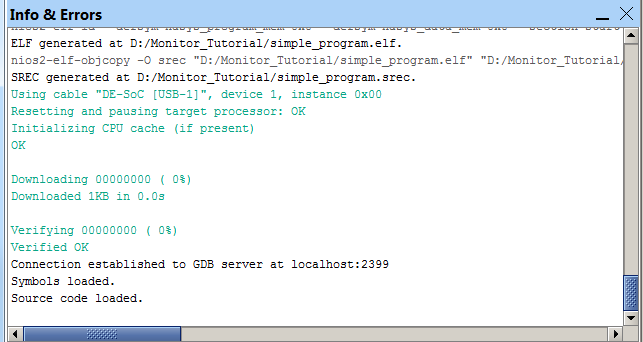
\includegraphics[scale=.8]{screenshots/figure12.png}
   \end{center}
   \caption{Compilation and loading messages.} 
	 \label{fig:12}
\end{figure}

After successfully completing this step, the Monitor Program display should look similar to Figure~\ref{fig:13}. At this point the
processor is halted at the first instruction of the program that
has to be executed, which is highlighted in yellow shading.
The main part of the display in Figure~\ref{fig:13} is called the
{\it Disassembly} window. 
It shows the machine code for the assembled program,
as well as the addresses of memory locations in which the
instructions are loaded. It also shows the assembly-language
version of the assembled instructions.

\begin{figure}[H]
   \begin{center}
      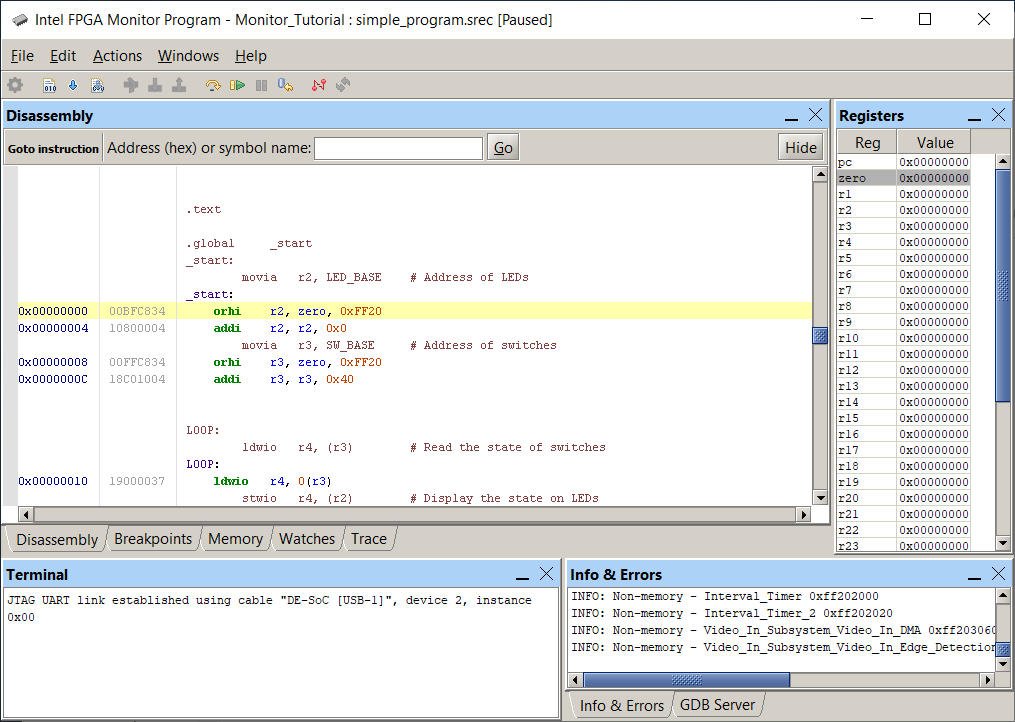
\includegraphics[scale=.57]{screenshots/figure13.png}
   \end{center}
   \caption{The Monitor Program window after loading the program.} 
	 \label{fig:13}
\end{figure}

\newpage
Most instructions in a Nios II assembly-language source program
are assembled into directly-corresponding machine instructions in
the object code that is loaded into the memory for execution.
But, this is not the case with all instructions. The Nios II
assembly language provides numerous {\it pseudo-instructions},
which are often replaced by actual instructions that look
quite different but have the same effect when executed.
For instance, the pseudo-instruction
\begin{center}
movia~~~r3, SWITCHES
\end{center}
\noindent
loads into processor register r3 the memory address of the I/O
data register that is connected to the slider switches on the
board. The required address is 32 bits long. However, immediate
operands in Nios II Load instructions can be at most 16 bits
long. Therefore, as seen in Figure~\ref{fig:13}, 
the second \texttt {movia} instruction is replaced with two
instructions. The instruction 
\begin{center}
orhi~~~r3, zero, 0xFF20
\end{center}
\noindent
places the immediate operand 0xFF20 into the high-order 16 bits
of register r3 and leaves the low-order 16 bits equal to zero.
The instruction
\begin{center}
addi~~~r3, r3, 0x40
\end{center}
\noindent
changes the low-order 16 bits into 0x40, thus completing in
register r3 the required address 0xFF200040.
Information about Nios~II instructions and
pseudo-instructions can be found in the tutorial
\emph{Introduction to the Intel Nios~II Soft Processor}, available in the University Program section of Intel's website.


\subsubsection{Compilation Errors}

During the process of developing software, it is likely that compilation errors will be 
encountered. Error messages from the Nios II assembler or from
the C compiler are displayed in the \textsf{Info \& Errors}
window. To see an example of a compiler error message, edit
the file {\it simple\_program.s}, which is in the project's directory, and replace the Branch instruction mnemonic 
\texttt {br} with \texttt {b}.
Recompile the project to see the error shown in Figure~\ref{fig:14}. 
The error message indicates the type of error and it gives the
line number in the file where the error was detected. Fix the
error, and then compile and load the program again.

\begin{figure}[H]
   \begin{center}
      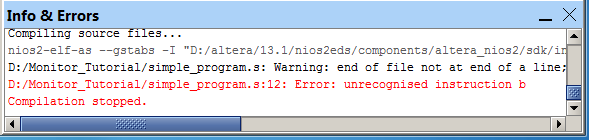
\includegraphics[scale=1]{screenshots/figure14.png}
   \end{center}
   \caption{An example of a compiler error message.} 
	 \label{fig:14}
\end{figure}


%%%%%%%%%%%%%%%%%%%%%%%
%%% Running the Program
\subsection{Running the Program}
%\label{sec:run_program}

As mentioned in the previous section, the processor is halted at
the first instruction after the program has been loaded. 
To run the program, select the \textsf{Actions > Continue} menu
item or click the 
\includegraphics{toolbar/continue.png} icon.  The {\it simple\_program} displays the current values of
DE1-SoC board's slider switches on the red LEDs.
The \textsf{Continue} command runs the program indefinitely.
To force the program to halt,
select the \textsf{Actions > Stop} command, or click the

\includegraphics{toolbar/stop.png} icon. This command causes the
processor to halt at the instruction to be executed next, and
returns control to the Monitor Program. 

Figure~\ref{fig:15} shows an example of what the display may look like when
the program is halted by using the {\sf Stop} command. 
The display highlights in yellow the next program instruction to
be executed, which is at address \texttt {0x00000014},
and highlights in red the values in the processor
registers that have changed since the last program stoppage.
Other screens in the Monitor Program are also updated, which will
be described in later parts of this tutorial.

\begin{figure}[H]
   \begin{center}
      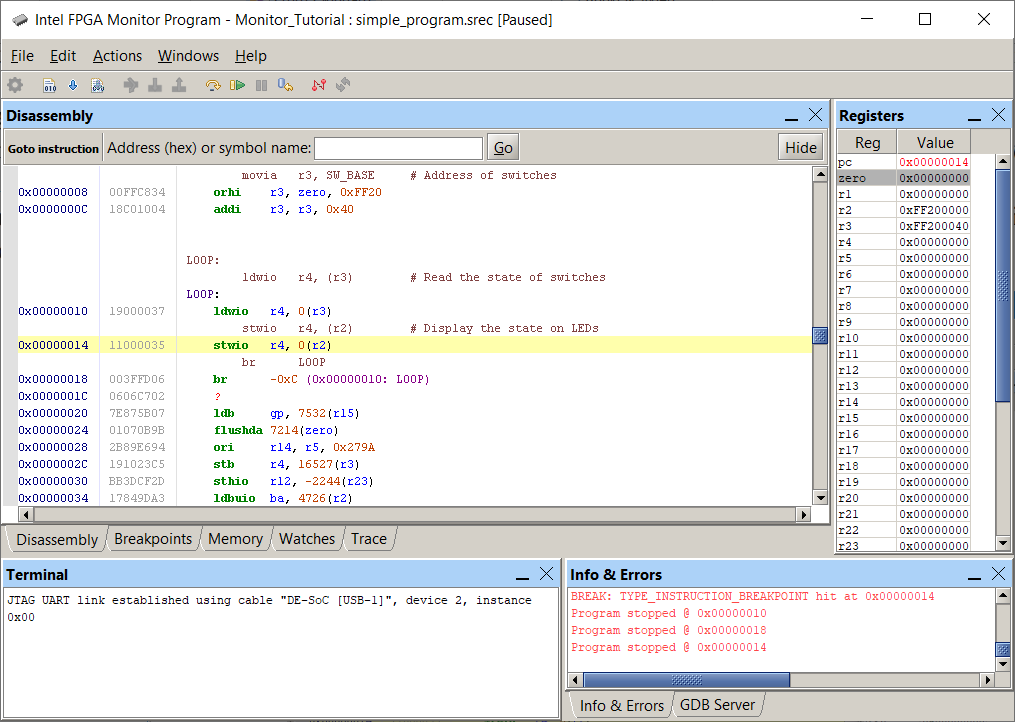
\includegraphics[scale=0.6]{screenshots/figure15.png}
   \end{center}
   \caption{The Monitor Program display after the program has been stopped.} 
	 \label{fig:15}
\end{figure}


%%%%%%%%%%%%%%%%%%%%%%%%%%%%%%%%
%%% Using the Disassembly Window
\subsection{Using the Disassembly Window}
%\label{sec:disassembly_window}

In Figure~\ref{fig:15}, the Disassembly window shows the machine
instructions for our program.
The leftmost column in the window gives the memory addresses,
the middle column displays the machine code at these addresses,
and the rightmost column shows both the original source code for
the instruction, in a brown color, and the disassembled view of
the machine code that is stored in memory, in a green color.

The Disassembly window can be configured to display less information on the screen, such as 
not showing the assembly-language instructions or not showing the machine encoding of the instructions. These choices can 
be made by right-clicking on the Disassembly window and selecting
the appropriate menu item, as indicated in Figure~\ref{fig:16}.

\begin{figure}[H]
   \begin{center}
      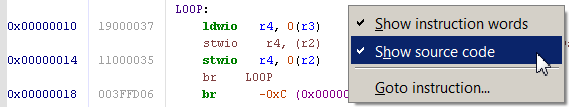
\includegraphics[scale=1]{screenshots/figure16.png}
   \end{center}
   \caption{Display options for the Disassembly window.} 
	 \label{fig:16}
\end{figure}

Different parts of memory can be displayed by scrolling, 
using either the vertical scrollbar on the right side of the Disassembly window or a mouse scroll wheel.
It is also possible to go to a different region of memory by 
using the \textsf{Goto instruction} panel 
at the top of the Disassembly window, or by using the command \textsf{Actions > Goto instruction}.  The instruction address
provided for the {\sf Goto} command must be a multiple of four,
because Nios II instructions are word-aligned. 

%%%%%%%%%%%%%%%
%%% Single step
\subsection{Single Stepping Program Instructions}

When debugging a program, it is often very useful to be able
to single step through the program and observe the effect of
executing each instruction. 
The Monitor Program has the ability to perform single-step
operations. Each single step consists of executing a single
machine instruction and then returning control to the Monitor
Program. If the source code of the program being debugged is
written in the C language, then each individual single step will
still correspond to one assembly-language (machine) instruction
generated from the C code. 

The single-step operation is invoked by selecting the
\textsf{Actions > Single step} menu item or by clicking on the 
\includegraphics{toolbar/singlestep.png} icon. The 
instruction that is executed by the processor is the
one highlighted in yellow in the \textsf{Disassembly} window.
Consider our {\it simple\_program} example. You can go to the
first instruction of the program, which has the label 
{\it \_start}, by selecting \textsf{Actions > Restart} 
menu item or by clicking  
the 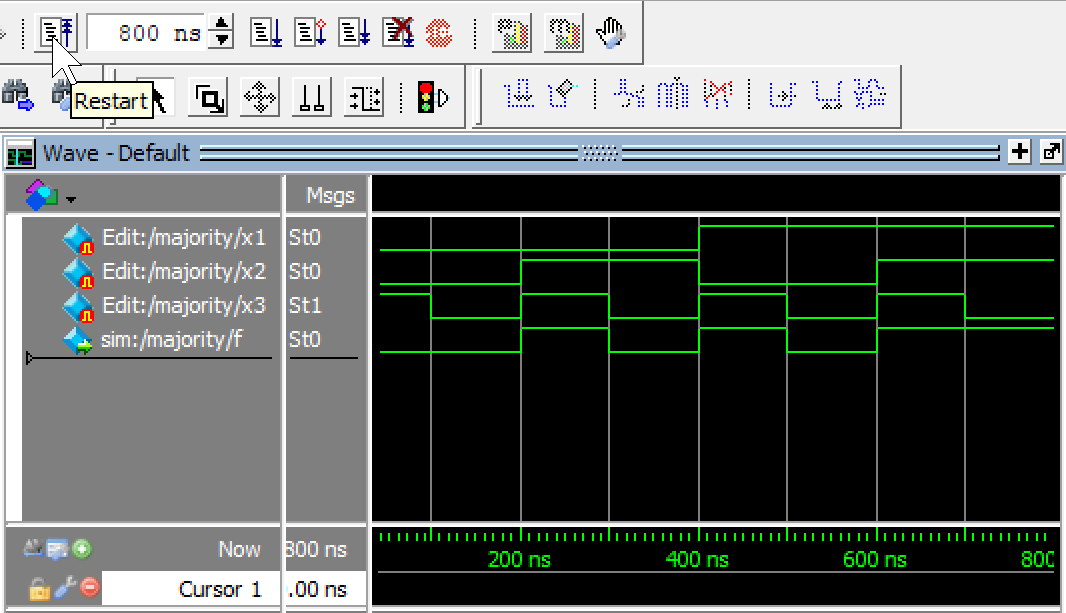
\includegraphics{toolbar/restart.png} icon. If the program is
running, it must first be halted before the restart 
command can be performed.
The restart command loads into the Program Counter the address of
the first instruction, thus causing the execution to start at
this point in the program.
Now, single step through the program and observe the displayed 
changes. Note that the register values are indicated in red when
they change as a result of executing the last instruction.

In a program that contains subroutines it is possible to step
over an entire subroutine by using the
{\sf Step Over Subroutine} command in the {\sf Actions} menu.
This command performs a normal single step, unless the current
instruction is a Call instruction, in which case the program will
run until the called subroutine is completed.

%%%%%%%%%%%%%%%%%%%%%
%%% Using Breakpoints
\subsection{Using Breakpoints}
%\label{sec:inst_breakpoints}

An {\it instruction breakpoint} provides a means of stopping the
execution of a program when it reaches an instruction at a
specific address.  The procedure for setting a breakpoint is:

\begin{enumerate}
\item In the Disassembly window, scroll to display the instruction that will have the breakpoint. For example, 
in the window in Figure~\ref{fig:15} scroll
to the Branch instruction at address 0x00000018. 

\item Click on the gray bar to the left of the address
0x00000018. As illustrated in Figure~\ref{fig:17},
the Monitor Program displays a red dot next to the address
to show that a breakpoint has been set. 
Clicking the same location again removes the breakpoint.
\end{enumerate}

\begin{figure}[H]
   \begin{center}
      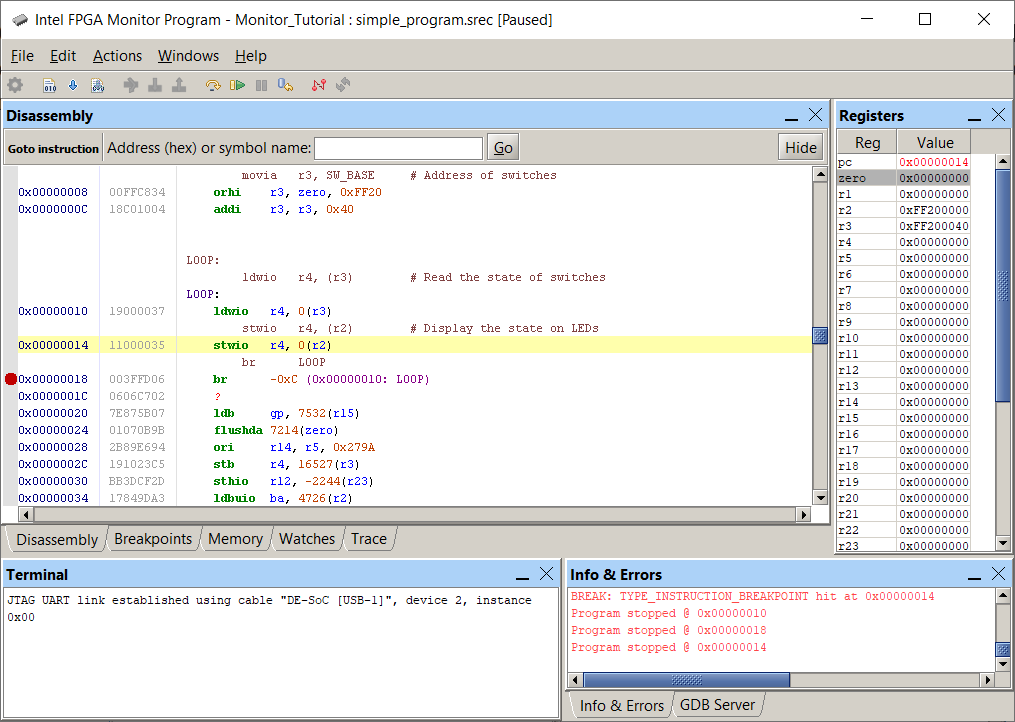
\includegraphics[scale=0.6]{screenshots/figure17.png}
   \end{center}
   \caption{Setting a breakpoint.} 
	 \label{fig:17}
\end{figure}

Once the instruction breakpoint has been set, run the program.
The breakpoint will trigger when the Program Counter value equals 0x00000018. Control then returns to the Monitor Program,
and the Disassembly window highlights in a yellow color the
instruction at the breakpoint. A corresponding message is shown
in the {\sf Info \& Errors} pane.

Some versions of the Nios~II processor support other types of
breakpoints in addition to instruction breakpoints. Other types
of breakpoints are described in Appendix A.

%%%%%%%%%%%%%%%%%%%%%%%%%%%%%%%%%%%%%%%%%%
%%% Examining and Changing Register Values
\subsection{Examining and Changing Register Values}

The \textsf{Registers} window on the right-hand side of the
Monitor Program display shows the values of processor registers.
It also allows the user to edit most of the register values. 
The number format in which the register values are displayed
can be changed by right-clicking in the \textsf{Registers}
window and selecting the desired format, as illustrated in 
Figure~\ref{fig:18}.

\begin{figure}[H]
   \begin{center}
      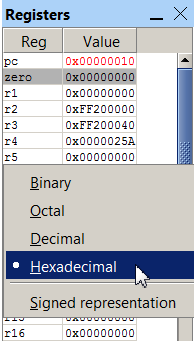
\includegraphics[scale=1]{screenshots/figure18.png}
   \end{center}
   \caption{Setting the number format for displaying register values.} 
	 \label{fig:18}
\end{figure}

Each time program execution is halted, the Monitor Program
updates the register values and highlights any changes in red.
The user can edit the register values while the program is
halted. Any edits made are visible to the processor when the
program's execution is resumed.

As an example of editing a register value, set the slider
switches on the DE1-SoC board to some pattern of 0s and 1s.
Run the {\it simple\_program} and observe that the LEDs display
the selected pattern. Next, stop the execution of the program
and set a breakpoint at the Store instruction
at address \texttt{0x00000014}. Run the program and
after the execution stops at the breakpoint, observe that the
value in register r4 corresponds to the current setting of the
slider switches. 
Now,  as indicated in Figure~\ref{fig:19}, double-click on the contents of
register r4 and change them to the value FFF.  
Press \textsf{Enter} on the computer keyboard, or click away from
the register value to apply the edit. 
Then, single-step the program to see that all LEDs will be
turned on. 

\begin{figure}[H]
   \begin{center}
      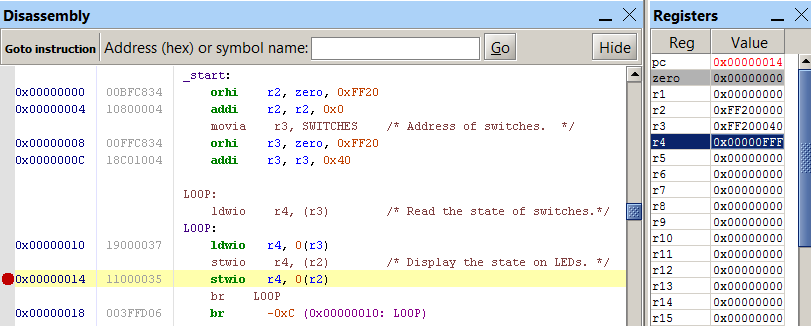
\includegraphics[scale=1]{screenshots/figure19.png}
   \end{center}
   \caption{Editing a register value.} 
	 \label{fig:19}
\end{figure}


%%%%%%%%%%%%%%%%%%%%%%%%%%%%%%%%%%%%%%%%%%
%%% Examining and Changing Memory Contents
\subsection{Examining and Changing Memory Contents}

The Memory window, depicted in Figure~\ref{fig:20}, displays the contents
of the system's memory space and allows the user to edit memory
values. The leftmost column in the window gives a memory address,
and the numbers at the top of the window represent hexadecimal
address offsets from that corresponding address. 

\begin{figure}[H]
   \begin{center}
      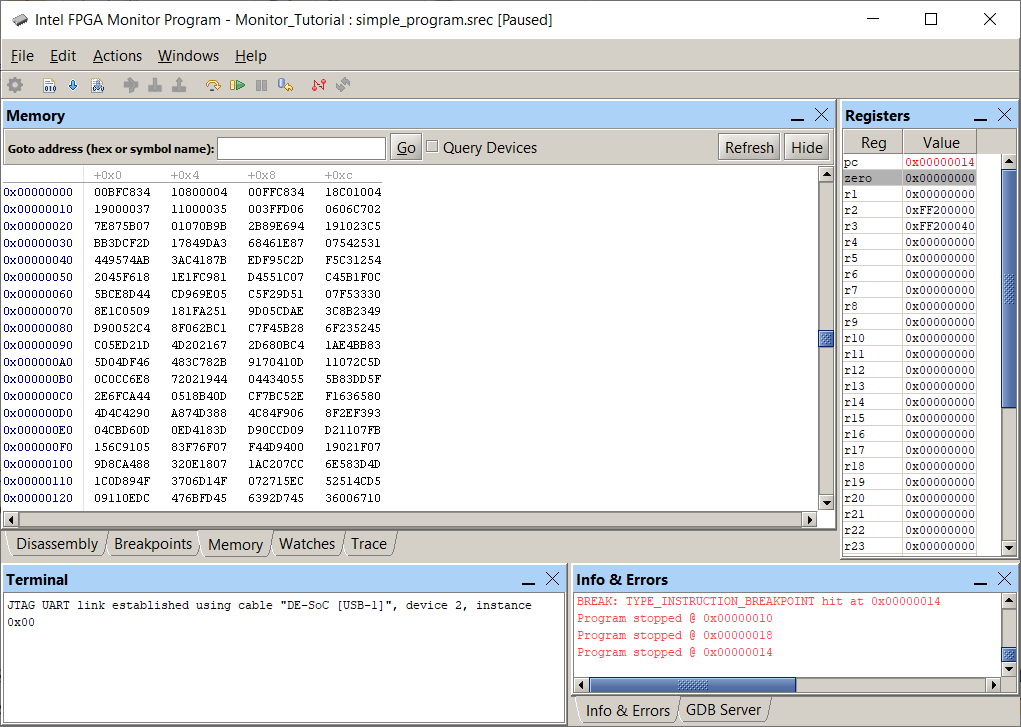
\includegraphics[scale=0.57]{screenshots/figure20.png}
   \end{center}
   \caption{The Memory window.} 
	 \label{fig:20}
\end{figure}

In this figure, the address of the second word in the
second row is \texttt{0x00000010 + 0x4 = 0x00000014}.
The displayed contents of this memory location are 0x11000035,
which is the machine code for the instruction
\begin{center}
stwio~~~~r4, 0(r2)
\end{center}

If a program is running, the data values displayed in the
Memory window are not updated. But, when the program is stopped,
the data values are automatically updated. They can also be
updated by pressing the {\sf Refresh} button. 
By default, the Memory window shows only the contents of memory
devices, and does not display any values from memory-mapped I/O devices. To cause the window to display memory-mapped
I/O locations, click on the check mark beside 
{\sf Query Devices}, and then click 
{\sf Refresh}. For example, set the slider switches to some
pattern, press {\sf Refresh}, enter the address 
\texttt{0xFF200040} into the {\it goto address} box and then press {\sf Go}. Figure~\ref{fig:21} shows the
display we obtained when choosing the pattern 0x30F.

\begin{figure}[H]
   \begin{center}
      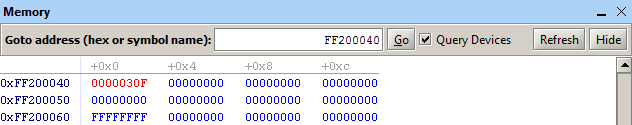
\includegraphics[scale=1]{screenshots/figure21.png}
   \end{center}
   \caption{Displaying the I/O locations.} 
	 \label{fig:21}
\end{figure}

The color of a memory word displayed depends on whether that
location corresponds to an actual memory device, a memory-mapped
I/O device, or is not mapped at all in the system. 
A memory location that corresponds to a memory device will be 
colored black, as in Figure~\ref{fig:20}. Memory-mapped I/O is shown in
blue color, and a non-mapped address is
shown in grey. If a memory location changed value since it was previously displayed, then
that memory location is shown in a red color.

Similar to the Disassembly window, it is possible to view
different memory regions by scrolling using the vertical scroll
bar on the right, or by using a mouse scroll wheel.
There is also a \textsf{Goto address} panel, which is
analogous to the \textsf{Goto instruction} panel discussed in Section 3.4. Note that in Figure~\ref{fig:21} we reached the I/O device
by typing the address \texttt{FF200040} in this panel.
  
As an example of editing a memory value, go to address
\texttt{FF200000} which is the address of LEDs.
Double-click on the memory word at this address 
and type the data value FFF. Press \textsf{Enter} on
the computer keyboard, or click away from the memory word to
apply the edit. This should cause all LEDs to be turned on. 

When accessing an I/O device, some reads may be destructive.
Namely, after some register in the I/O interface is read, its
contents may no longer be valid. Therefore, it is not
appropriate to read all I/O registers when refreshing the
information in the Memory window. Instead, it is prudent to read
only the registers that are of specific interest. This can be
accomplished  by left-clicking on the address of interest,
then right-clicking and selecting {\sf Read Selected Address Range} to update the displayed contents. Several
consecutive addresses can be selected by clicking on the first
address and dragging across the other addresses.

It is possible to change the appearance of the Memory window in a
number of ways, such as displaying data as bytes, half-words or
words. 
The Memory window provides additional features that are described
in more detail in Appendix A of this document.
 

%%%%%%%%%%%%%%%%%%%%%%%
%%% Working with Project Files
\section{Working with Project Files}

Project files store the settings for a particular project, 
such as the specification of a hardware system and program source
files. A project file, which has the filename 
extension {\it .amp}, is stored into a project's directory when
the project is created. 

The Monitor Program provides the following commands, under the
{\sf File} menu, for working with project files:

\begin{enumerate}
    \item {\sf New Project}: Presents a series of screens that are used to create a new project.
    \item {\sf Open Project}: Displays a dialog to select an
existing project file and loads the project.
    \item {\sf Open Recent Project}:  Displays the five most recently used project files, and allows these projects to be
reopened.
    \item {\sf Save Project}: Saves the current project's
settings after they have been modified by using 
the {\sf Settings} command.
\end{enumerate}

\subsection{Modifying the Settings of an Existing Project}

After a project has been created, it is possible to modify many
of its settings, if needed. This can be done by clicking
on the menu item {\sf File > Edit Project > System Settings} in the Monitor
Program.
This action will display the existing system settings for the
project, and allow them to be changed. Similarly, the program
settings for the project can be displayed and modified by using
the command {\sf File > Edit Project > Program Settings}. To change
these settings, the Monitor Program has to first be disconnected
from the system being debugged. This can be done by using the
command {\sf Actions > Disconnect}, or by clicking the

\includegraphics{toolbar/disconnect.png} icon.


%%%%%%%%%%%%%%%%%%%%%%%%%%%%%%%%%%%%%
%%% Using an Evaluation License
\section{Using the Monitor Program with a Nios\textsuperscript{\textregistered} II Evaluation License}
\label{sec:custom_system}

In our discussion of Figure~\ref{fig:11} in Section 3.1,
we showed how the Monitor Program can be used to download a
prebuilt Nios~II hardware system onto an FPGA board, when the
Nios~II processor has a license. It is also possible to use the
Monitor Program to debug hardware systems in which the Nios~II
processor includes only an evaluation license. In this case
it is necessary to download the hardware system onto the FPGA
board by using the {\it Programmer} tool provided in the 
Quartus Prime software, rather than using the Monitor Program for
this purpose. The Quartus Prime Programmer tool provides a pop-up
window, shown in Figure~\ref{fig:22}, which indicates activation of
the evaluation license for the Nios~II processor. 
This pop-up window has to remain open in order to maintain the
evaluation license for Nios~II. As long as the pop-up
window remains open, the Monitor Program can be used to compile
and download software programs into the hardware system.
~\\
~\\

\begin{figure}[H]
   \begin{center}
      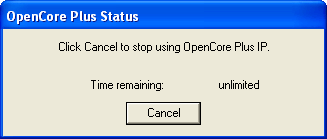
\includegraphics[scale=1]{screenshots/figure22.png}
   \end{center}
   \caption{The Quartus Prime Programmer pop-up window.} 
	 \label{fig:22}
\end{figure}

%%%%%%%%%%%%%%%%%%%%%%
%%% Using the Terminal
\section{Using the Terminal Window}

Monitor Program's \emph{Terminal} window supports
text-based input and output. To see its operation, create
a new Monitor Program project, called {\it Monitor\_Terminal}.
When creating the project, follow the same steps shown for the
{\it Monitor\_Tutorial} project, which were described in 
Section 3.1. For the screen shown in Figure~\ref{fig:7} set the program
type to {\sf Assembly Program}, and select the
sample program named {\it JTAG* UART}. The source code file 
for that program is called {\it JTAG\_UART.s}.  
It communicates using memory-mapped I/O with the JTAG UART in 
the DE1-SoC Computer that is selected as 
the {\sf Terminal device} in the screen of Figure~\ref{fig:9}.

Compile, load and run the program. The Monitor Program
window should appear as shown in Figure~\ref{fig:23}. 
Click the mouse inside the Terminal window. Now, any characters
typed on the computer keyboard are sent by the Monitor Program to
the JTAG UART. These characters are shown in the Terminal window
as they are typed, because the {\it JTAG\_UART.s} program echoes
the characters back to the Terminal window.

\begin{figure}[H]
   \begin{center}
      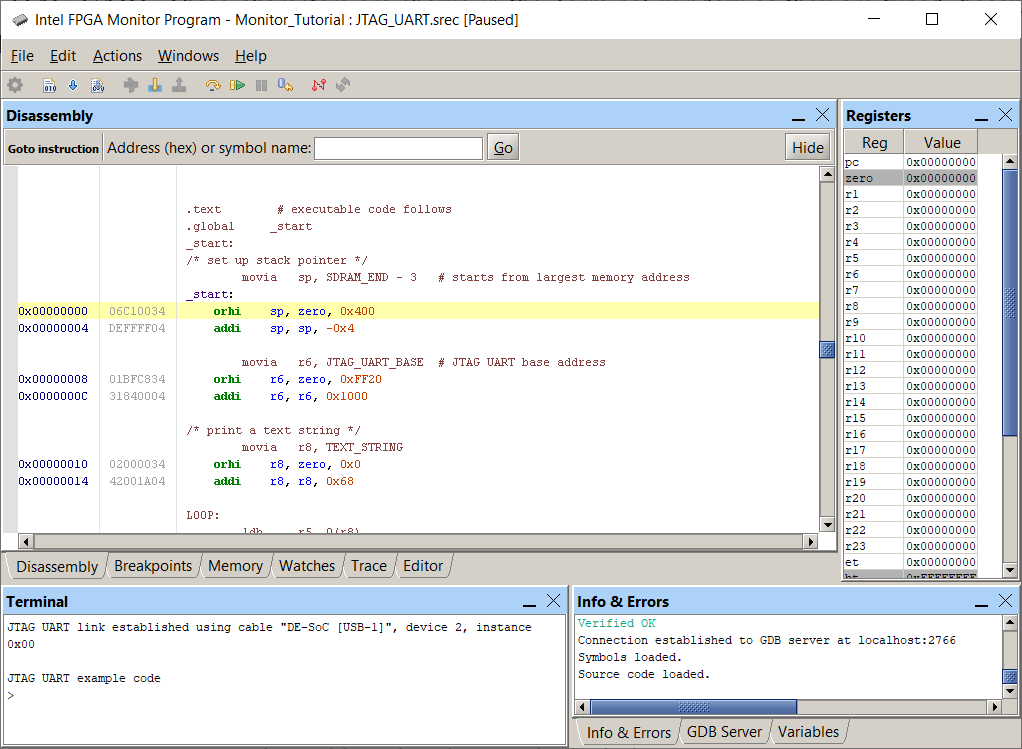
\includegraphics[scale=.55]{screenshots/figure23.png}
   \end{center}
   \caption{Using the Terminal window.} 
	 \label{fig:23}
\end{figure}

\newpage
The Terminal window supports a subset of the control character
commands used for a de facto standard terminal, called 
the {\it VT100*}.
The supported commands are listed in Table~\ref{tbl:1}.
In this table \texttt{<ESC>} represents the ASCII character 
with the code \texttt{0x1B}.

\begin{table}[H]
    \centering
    \begin{tabular}{|l|p{4in}|}
        \hline
        Character Sequence&Description\\
        \hline
        \hline
        \texttt{<ESC>[2J}&Erases everything in the Terminal window\\
        \hline
        \texttt{<ESC>[7h}&Enable line wrap mode\\
        \hline
        \texttt{<ESC>[7l}&Disable line wrap mode\\
        \hline
        \texttt{<ESC>[\emph{\#}A}&Move cursor up by \emph{\#} rows or by one row if \emph{\#} is not specified\\
        \hline
        \texttt{<ESC>[\emph{\#}B}&Move cursor down by \emph{\#} rows or by one row if \emph{\#} is not specified\\
        \hline
        \texttt{<ESC>[\emph{\#}C}&Move cursor right by \emph{\#} columns or by one column if \emph{\#} is not specified\\
        \hline
        \texttt{<ESC>[\emph{\#}D}&Move cursor left by \emph{\#} columns or by one column if \emph{\#} is not specified\\
        \hline
        \texttt{<ESC>[\emph{$\#_1$};\emph{$\#_2$}f}&Move the cursor to row \emph{$\#_1$} and column \emph{$\#_2$}\\
        \hline
        \texttt{<ESC>[H}&Move the cursor to the home position (row 0 and column 0)\\
        \hline
        \texttt{<ESC>[s}&Save the current cursor position\\
        \hline
        \texttt{<ESC>[u}&Restore the cursor to the previously saved position\\
        \hline
        \texttt{<ESC>[7}&Same as \texttt{<ESC>[s}\\
        \hline
        \texttt{<ESC>[8}&Same as \texttt{<ESC>[u}\\
        \hline
        \texttt{<ESC>[K}&Erase from current cursor position to the end of the line\\
        \hline
        \texttt{<ESC>[1K}&Erase from current cursor position to the start of the line\\
        \hline
        \texttt{<ESC>[2K}&Erase entire line\\
        \hline
        \texttt{<ESC>[J}&Erase from current line to the bottom of the screen\\
        \hline
        \texttt{<ESC>[1J}&Erase from current cursor position to the top of the screen\\
        \hline
        \texttt{<ESC>[6n}&Queries the cursor position. A reply is sent back in the format \texttt{<ESC>[\emph{$\#_1$};\emph{$\#_2$}R},
            corresponding to row \emph{$\#_1$} and column \emph{$\#_2$}.\\
        \hline
    \end{tabular}
    \caption{VT100 commands supported by the Terminal window.} 
		\label{tbl:1}

\end{table}

%%%%%%%%%%%%%%%%%%%%%%
%%% Using C code
\section{Using C Programs}
%\label{sec:c_code}

C programs are used with the Monitor Program in a similar way as
assembly-language programs. To see an example of a C program,
create a new Monitor Program project called 
{\it Monitor\_Terminal\_C}. Use the same settings as for the
{\it Monitor\_Terminal} example, but set the program type for
this project to {\sf C Program}.
Select the C sample program called {\it JTAG UART}.  
As illustrated in Figure~\ref{fig:24}, this program includes a C source
file named {\it JTAG\_UART.c}; it has the same functionality as
the assembly-language code used in the previous example. 
Compile and run the program to observe its behavior.

\begin{figure}[H]
   \begin{center}
      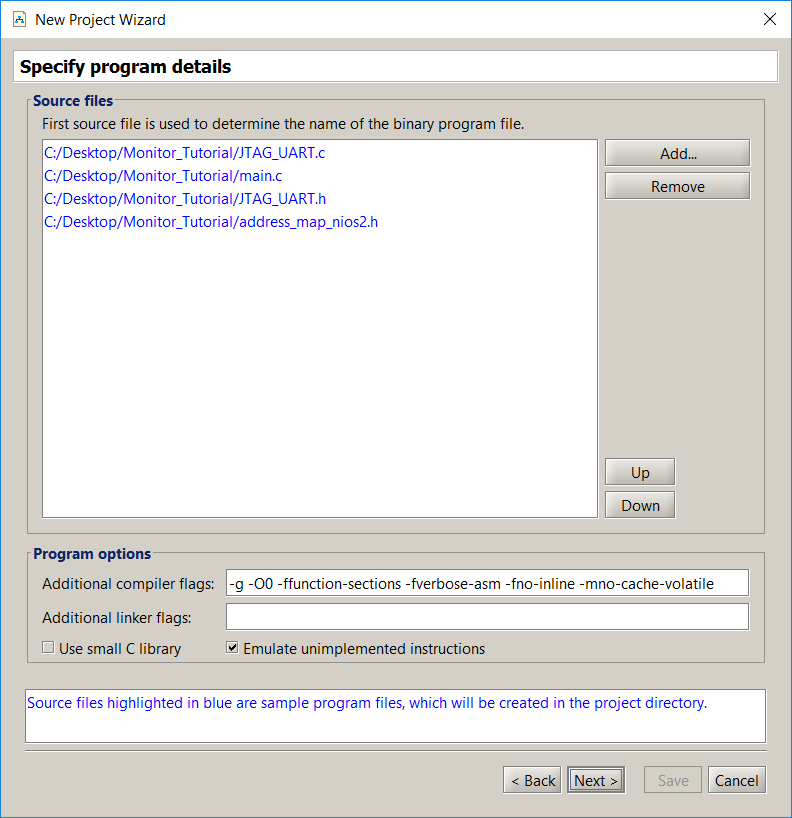
\includegraphics[scale=0.5]{screenshots/figure24.png}
   \end{center}
   \caption{Settings for a C program.} 
	 \label{fig:24}
\end{figure}

The C code in {\it JTAG\_UART.c} uses memory-mapped I/O to
communicate with the JTAG UART. Alternatively, it is possible to
use functions from the standard C library {\it stdio.h}, such as
{\it putchar}, {\it printf}, {\it getchar}, and {\it scanf} for
this purpose.  Using these library functions impacts the size of
the Nios~II executable code that is produced when the C program
is compiled, by about 30 to 64 KBytes, depending on
which functions are needed.  It is possible to minimize the size
of the code generated for this library by checking the box labeled {\sf Use small C library} in 
Figure~\ref{fig:24}. When this option is used the
library has reduced functionality. 
Some limitations of the small C library include: 
no floating-point support in the output routines, 
such as {\it printf}, and no support for input routines, 
such as {\it scanf} and {\it getchar}.

In Figure~\ref{fig:24} the option {\sf Emulate unimplemented instructions}
is checked. This option causes the C compiler to include code for
emulating any operations that are needed to execute the C program
but which are not supported by the processor. For example, the
Nios~II Economy version does not include a {\it multiply}
instruction, but the C program may need to perform this
operation. By checking this option, a multiply instruction 
will be implemented in software (by using addition and shift
operations).
\newpage 

%%%%%%%%%%%%%%%%%%%%%%%%%
%% Source Level Debugging
\subsection{Source Level Debugging}
The Monitor program supports common source level debugging features such as step over, step into, 
step out, and visualizing variables. Using the JTAG UART sample program project you created in the previous section, 
go to the project settings ({\sf File > Edit Project }) and navigate to the {\it Program Settings} tab. 
In the {\it Compiler Flags} input box, ensure that the optimization level is set to 0, by replacing {\it -O, -O1, -O2, } 
or {\it -O3} flag with {\it -O0}. An optimization level of 0 allows the Monitor Program to read and display 
variables from memory. Figure~\ref{fig:25} shows the Monitor Program's text editor. The editor will be disabled
during the debug session, and re-enabled when the debug session is exited. Now save the project ({\sf File > Save Project}), 
and compile and load the program ({\sf Actions > Compile \& load}).

\begin{figure}[h]
   \begin{center}
      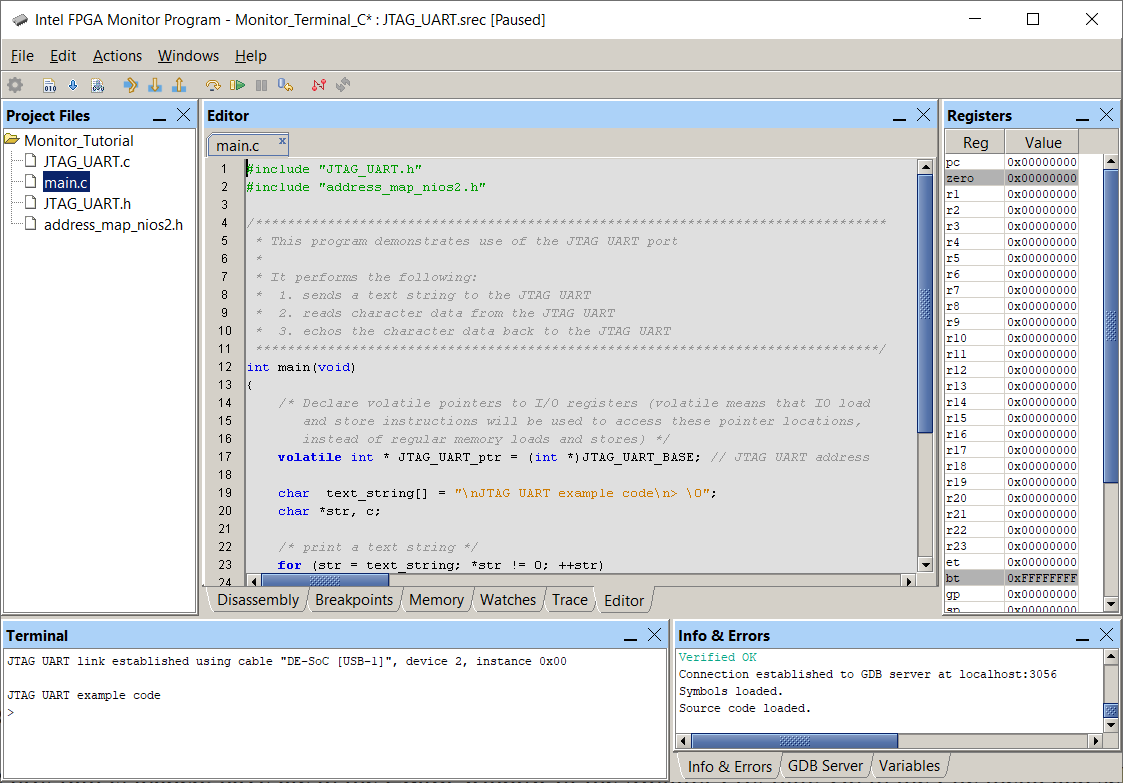
\includegraphics[scale=0.5]{screenshots/figure25.png}
   \end{center}
   \caption{The Monitor Program with a source file open in editor view.}
	 \label{fig:25}
\end{figure}

\subsubsection{Using Breakpoints}
Once the program is loaded, navigate to the {\sf Editor} window of the Monitor Program.
Go to the File menu and select {\sf File > Open...} to open the C source file which contains the {\it main} 
function of you program (most likely {\it main.c}).

Once the program is loaded, toggle the breakpoint at a line of source code by clicking on the numbers to the 
left of the source code text. If a breakpoint does not show up on the line similar to Figure~\ref{fig:26}, the line of source code 
likely does not correspond to an instruction. If this happens, try choosing a different line.

\begin{figure}[h]
   \begin{center}
      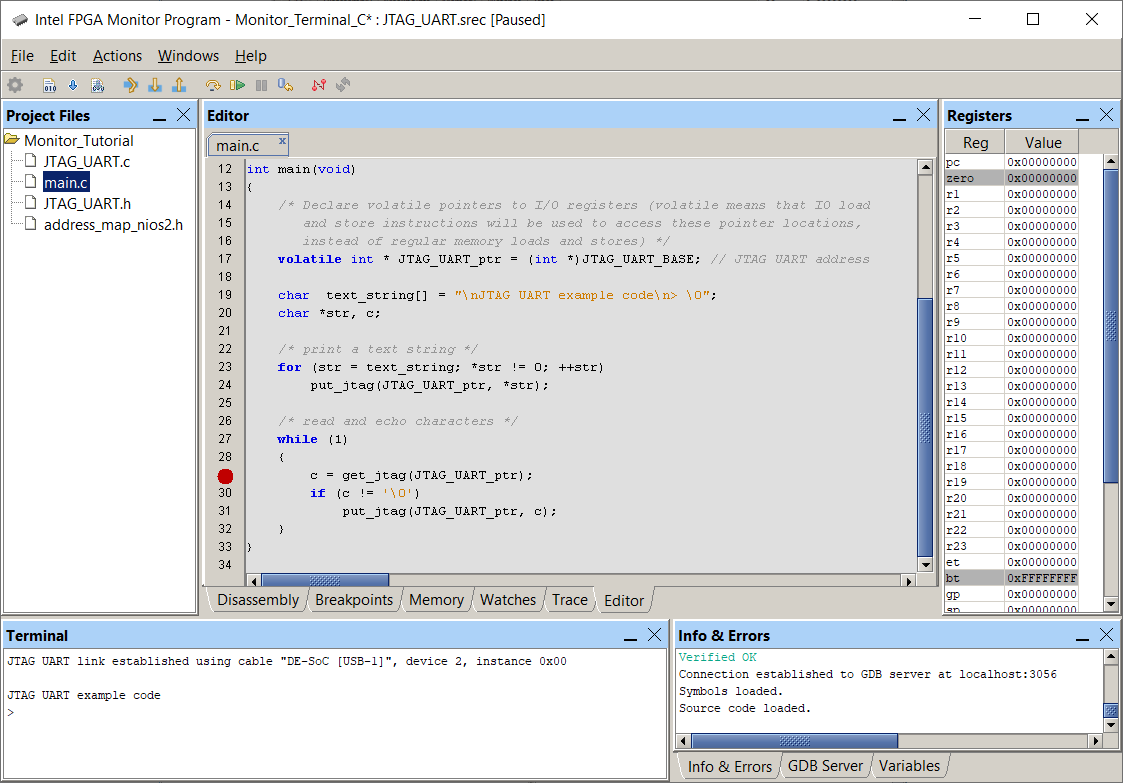
\includegraphics[scale=0.5]{screenshots/figure26.png}
   \end{center}
   \caption{Setting a breakpoint in the editor view.}
	 \label{fig:26}
\end{figure}

Once the breakpoint is set, continue the program by clicking the green arrow on the toolbar, or {\sf Actions > Continue}.
Once the program halts, the Monitor Program should look similar to Figure~\ref{fig:27}. In the Disassembly view the source level breakpoint 
is marked with a red square as in Figure~\ref{fig:28}. This differentiates source level breakpoints from instruction level breakpoints.\\

\begin{figure}[h]
   \begin{center}
      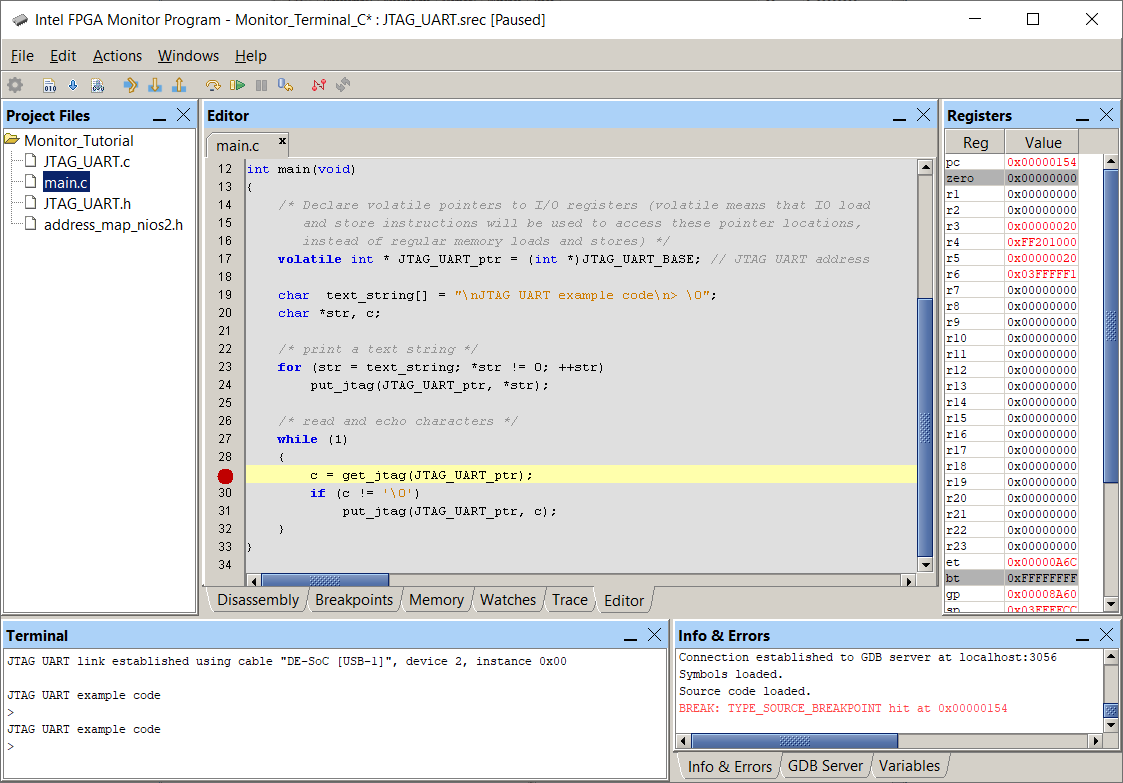
\includegraphics[scale=0.5]{screenshots/figure27.png}
   \end{center}
   \caption{Hitting a breakpoint in the editor view.}
	 \label{fig:27}
\end{figure}

\begin{figure}[h]
   \begin{center}
      
\includegraphics[scale=0.5]{screenshots/figure28.png}
   \end{center}
   \caption{Source level breakpoint in the disassembly view.}
	 \label{fig:28}
\end{figure}

\subsubsection{Source Level Debugging Actions}

\begin{figure}[h]
   \begin{center}
      
\includegraphics[scale=1]{screenshots/figure29.png}
   \end{center}
   \caption{Step Over, Step Into, Step Out toolbar icons}
	 \label{fig:29}
\end{figure}

Navigate back the editor view and perform a Step Into action by selecting {\sf Actions > Step Into}, or by using the main toolbar.
This will step to the next line of source code to be executed. If the program steps into a function in another file, the Monitor
Program will open the file in a new tab and highlight the line.

Next, perform a Step Out action by selecting {\sf Actions > Step Out}, or by using the main toolbar. This will step out of the current function 
by executing until the first line of source code after returning from the current function. The Monitor Program will print an error to the
{\sf Info \& Errors} window if it cannot step out of the current function. This may occur if the program is currently in the
{\it main} function, or if the function does not return. 
The step out function is only available for C programs, it is not available for assembly programs.

The Step Over action ({\sf Actions > Step Over}) moves to the next line of source code without stepping into functions. 
Execution will continue to the next line of source code inside the current function.


\subsubsection{Enabling and Disabling Source Level Debugging}
The source level debugging feature of the Monitor Program is a beta feature in the current release. The feature can be enabled and disabled at any point by going to the {\sf Edit} menu and selecting {\sf Edit > Enable Source Level Debugging}, or {\sf Edit > Disable Source Level Debugging}, depending on whether the feature is currently disabled or enabled respectively.


\subsubsection{Variable Values}

\begin{figure}[h]
   \begin{center}
      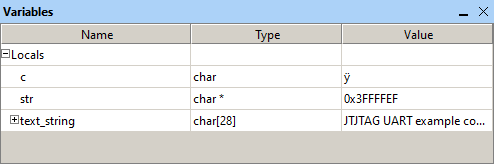
\includegraphics[scale=0.7]{screenshots/figure30.png}
   \end{center}
   \caption{Monitor Program Variable View.}
	 \label{fig:30}
\end{figure}

The Monitor Program's {\sf Variables} view is enabled when {\sf Enable Source Level Debugging}. It displays the value of C program variables when the program is halted.
Some variable types such as Arrays,  Typedefs, Structures and Unions will be expandable in the view. Use the {\sf +} button to 
expand and view the variables contents. Right clicking on a variable presents the options to jump to the declaration of the variable,
and the display format of the variable.\\

{\sf Go To Declaration} will open the file the variable is declared in and scroll to the declaration line number.\\
{\it Display As...} will change the format in which the variable is displayed.\\

Variable values are only available with an optimization level of \textbf{0} (gcc command line argument {\it -O0}). For instructions on how to change
the programs optimization level, see the first paragraph of this section.


\subsubsection{Setting the Optimization Level in Programs with Driver Support.}
To set the optimization level for a {\it Program with Driver Support} (or BSP), first create a TCL script in the base directory of the project (the same directory as your AMP project file). The TCl file should have a {\it .tcl} file extension, for example {\it config.tcl}. Open this file in a text editor and add the single line:\\
{\bf set\_setting hal.make.bsp\_cflags\_optimization -O0}\\
Where the argument {\it -O0} above is the desired optimization level. Now open the project settings in the Monitor Program and navigate to the {\it Program Settings} tab. In the {\it BSP settings Tcl script} input box (shown in Figure~\ref{fig:tclScript}) enter the path to the TCL script you just created, or use the {\it Browse} button to search for it.

\begin{figure}[H]
   \begin{center}
      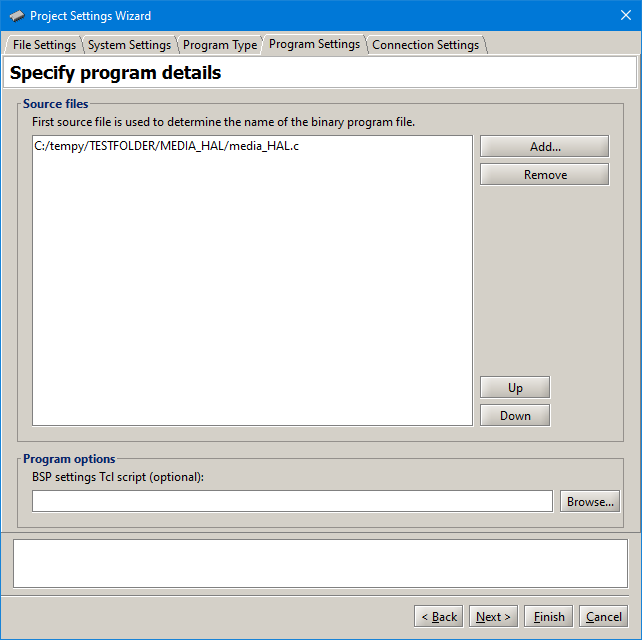
\includegraphics[scale=0.6]{screenshots/tclScript.png}
   \end{center}
   \caption{Adding a TCL script to a Program with Driver Support.}
	 \label{fig:tclScript}
\end{figure}

Click the {\it Finish} button to close the dialog and save and compile the project. The optimization level should be set for both the generated (BSP) files, as well as your project files.



%%%%%%%%%%%%%%%%%%%%%%%%%
%% Interrupts
\section{Using the Monitor Program with Interrupts}
%\label{sec:interrupts}

The Monitor Program supports the use of interrupts in Nios~II
programs. Two examples of interrupts are illustrated below, 
using assembly-language code and using C code.

\subsection{Interrupts with Assembly-Language Programs}

To see an example using interrupts with assembly-language code, 
create a new Monitor Program project
called {\it Monitor\_Interrupts}. When creating the new project
set the program type to assembly language and select the sample
program named {\it Interrupt Example}. 
Figure~\ref{fig:31} lists the source files for this sample program. 
The main program for the example is the file 
{\it interrupt\_example.s}, which initializes some I/O devices
and enables Nios~II interrupts. The other source files provide
the reset and exception handling for the program, and two interrupt service routines.

\begin{figure}[H]
   \begin{center}
      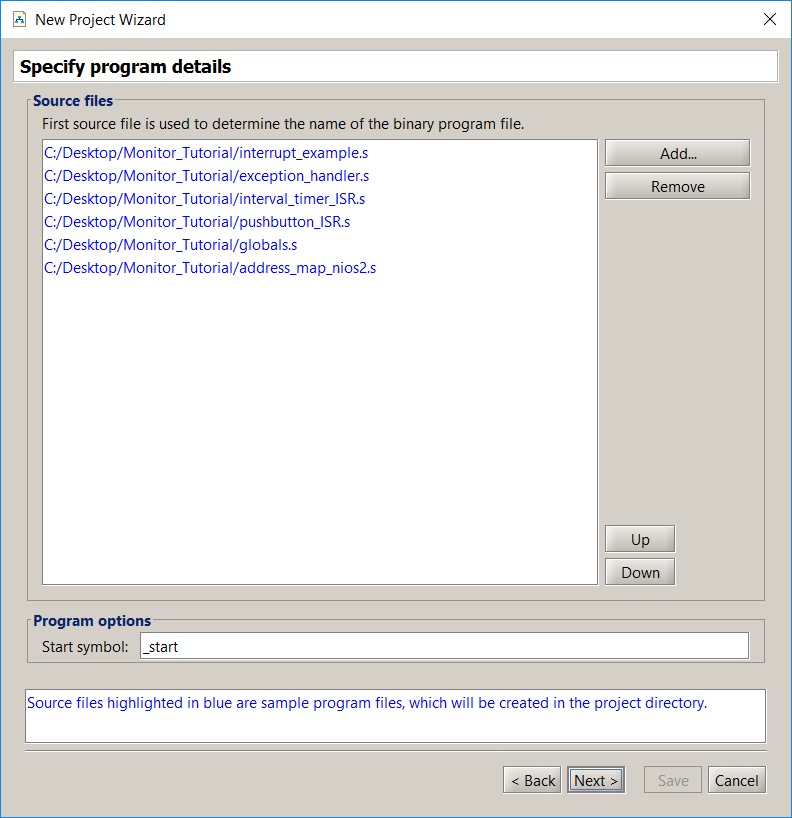
\includegraphics[scale=0.5]{screenshots/figure31.png}
   \end{center}
   \caption{The source files for the interrupt example.} 
	 \label{fig:31}
\end{figure}

 
Figure~\ref{fig:32} shows the memory settings for this program.
The reset vector of the Nios~II processor is at address 
\texttt{0x0} and the exceptions vector is at address 
\texttt{0x20}. Enough space has to be left between the exceptions
vector location and the text section of the program to
accommodate the exceptions processing code,
which corresponds to the assembly language code in the 
file {\it exception\_handler.s}. 
Starting the main program at address \texttt{0x200}, as shown
in the figure, leaves enough space to accommodate the exception
processing code for this example.

\begin{figure}[H]
   \begin{center}
      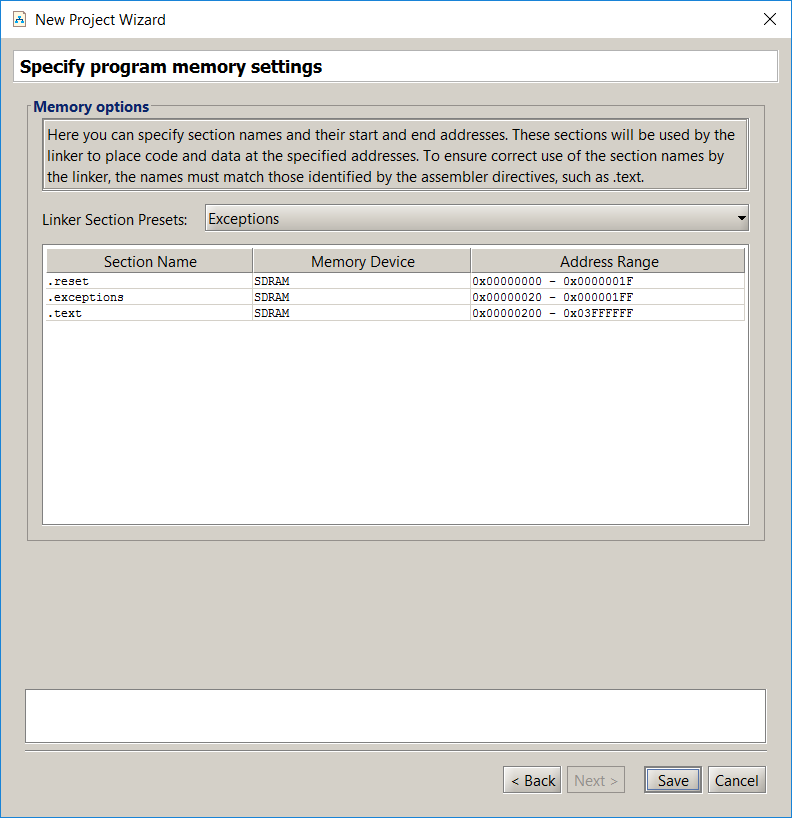
\includegraphics[scale=0.5]{screenshots/figure32.png}
   \end{center}
   \caption{Memory offset settings for the interrupt example.} 
	 \label{fig:32}
\end{figure}

Compile and load the program. Then, scroll the Disassembly window
to the label {\it EXCEPTION\_HANDLER}, which is at
address \texttt{0x00000020}.  
As illustrated in Figure~\ref{fig:33}, set a breakpoint at this address.
Run the program. When the breakpoint is reached, single step
the program a few more instructions to determine the cause of the
interrupt. The source of the interrupt is a circuit in the 
DE1-SoC Computer called the {\it interval timer}. This 
circuit provides the ability to generate an interrupt whenever a
specified time period elapses. Single step the program until the
processor enters the interrupt-service routine for the interval
timer. This routine first clears the timer register that caused
the interrupt, so that an interrupt request will not be raised
immediately again, and then performs other functions needed for
the program.

\begin{figure}[H]
   \begin{center}
      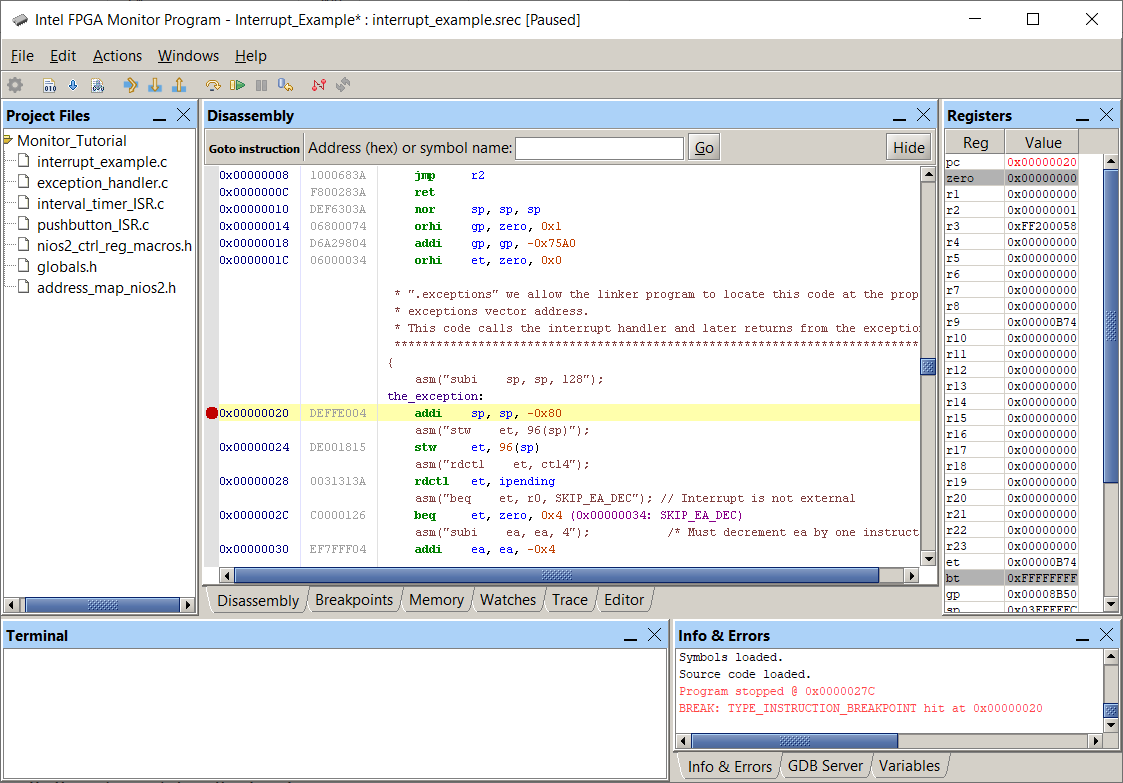
\includegraphics[scale=0.6]{screenshots/figure33.png}
   \end{center}
   \caption{The exception handler.} 
	 \label{fig:33}
\end{figure}

Finally, remove the breakpoint that was set earlier, at address
\texttt{0x00000020}, and then select the \textsf{Continue}
command to run the program. Observe that the program displays a
rotating pattern across the LED displays on the DE1-SoC board.
The direction of rotation can be changed by pressing the
pushbuttons KEY$_1$ or KEY$_2$ on the DE1-SoC board, and the
pattern can be changed to correspond to the
values of the slider switches by pressing KEY$_3$.  
%Pressing KEY$_0$ causes a reset of the Nios~II
%processor and returns control to the Monitor Program at the
%address \texttt{0x0}.

\subsection{Interrupts with C Programs}

To see an example of a C program that uses interrupts, create a
new project called {\it Monitor\_Interrupts\_C}.
When creating this project, set the program type to 
{\sf C Program} and select the sample program named 
{\it Interrupt Example}; this program gives C code that performs
the same operations as the assembly-language code in the previous
example. The source files for the C code are listed in 
Figure~\ref{fig:34}. The main program is given in the file 
{\it interrupt\_example.c}, and the other source files provide
the reset and exception handling for the C program, as well as
two interrupt-service routines.  Complete the steps for creating
the project, and then compile and load it.

Set a breakpoint at the address \texttt{0x00000020}, which is the
exception vector address for the Nios~II processor.  Also, scroll
the Disassembly window to the function called 
{\it interrupt\_handler}. As illustrated in Figure~\ref{fig:35}, set
another breakpoint at this address. Now, run the program to reach
the first breakpoint, at address \texttt{0x00000020}. 
The code at this address, which is found in the file
{\it exception\_handler.c}, reads the contents of a control
register in the Nios~II processor to determine if the interrupt
is caused by an external device, then saves registers on the
stack, and then calls the {\it interrupt\_handler} function.

\newpage
\begin{figure}[H]
   \begin{center}
      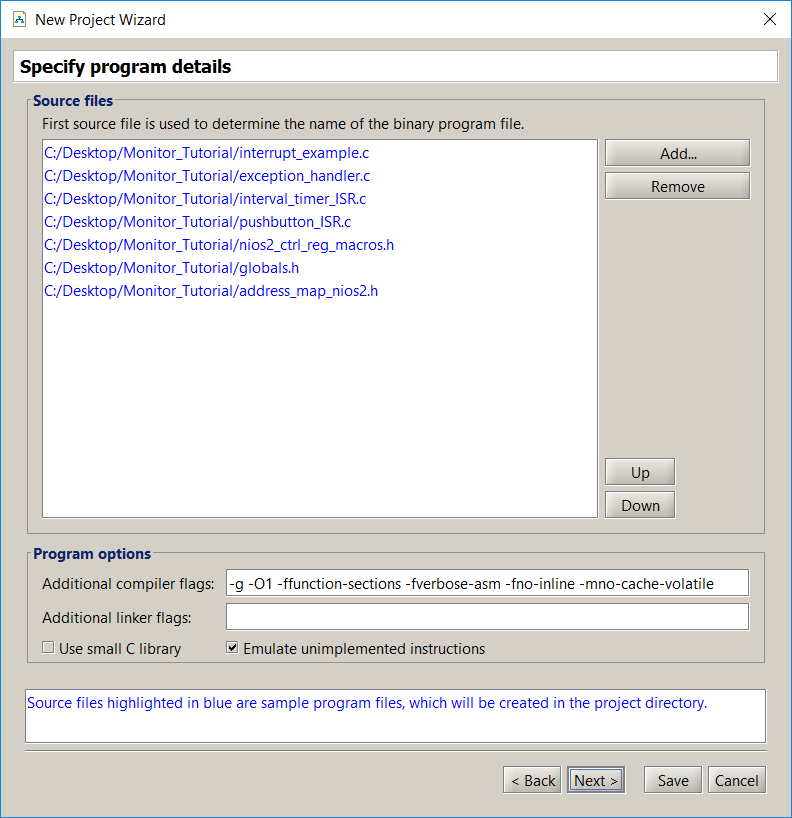
\includegraphics[scale=0.5]{screenshots/figure34.png}
   \end{center}
   \caption{The source files for the C code interrupt example.} 
	 \label{fig:34}
\end{figure}

~\\
~\\
\begin{figure}[H]
   \begin{center}
      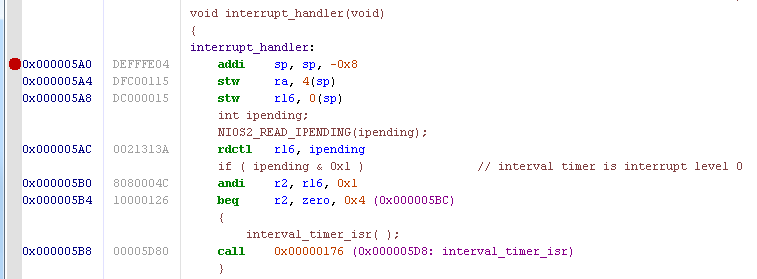
\includegraphics[scale=0.8]{screenshots/figure35.png}
   \end{center}
   \caption{The interrupt handler.} 
	 \label{fig:35}
\end{figure}


\newpage
Press {\sf Actions > Continue} in the Monitor Program to reach
the second breakpoint. Single stepping the program a few more
instructions shows that the interrupt is caused by the interval
timer in the DE1-SoC Computer, as discussed in the previous
example. Additional single stepping causes the processor to enter
the interrupt-service routine for the interval timer,
as depicted in Figure~\ref{fig:36}. This routine first clears the timer
register that caused the interrupt, and then performs other
functions needed for the program.
Finally, clear both breakpoints that were set earlier, at address
\texttt{0x00000020} and {\it interrupt\_handler}, and then run
the program; it displays a rotating pattern on the LED displays
of the DE1-SoC board, as discussed in the previous example.


\begin{figure}[H]
   \begin{center}
      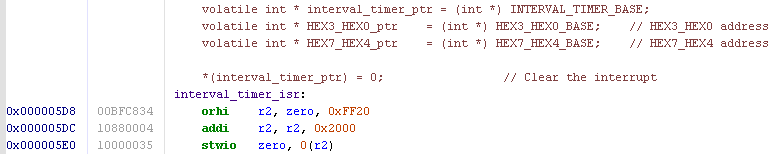
\includegraphics[scale=0.7]{screenshots/figure36.png}
   \end{center}
   \caption{The interrupt service routine for the interval timer.} 
	 \label{fig:36}
\end{figure}

%%%%%%%%%%%%%%%%%%%%%%%%%%%%%%%%%%%
%%% Working with Windows and Tabs
\section{Working with Windows and Tabs}

It is possible to rearrange the Monitor Program workspace by
moving, resizing, or closing the internal windows inside the main
Monitor Program window.

To move a particular window to a different location, click on the
window title or the tab associated with the window, and drag the
mouse to the new location. As the mouse is moved across the main
window, the dragged window will snap to different locations. 
To detach the dragged window from the main window, drag it beyond
the boundaries of the main window. 
To re-attach a window to the main window, drag the tab associated
with the window onto the main window.

To resize a window, hover the mouse over one of its borders, and
then drag the mouse. Resizing a window that is attached to the
main window will cause any adjacent attached windows to also
change in size accordingly.

To hide or display a particular window, use the {\sf Windows}
menu. To revert to the default window arrangement, simply exit
and then restart the Monitor Program. Figure~\ref{fig:37} shows an example
of a rearranged workspace.

\begin{figure}[H]
   \begin{center}
      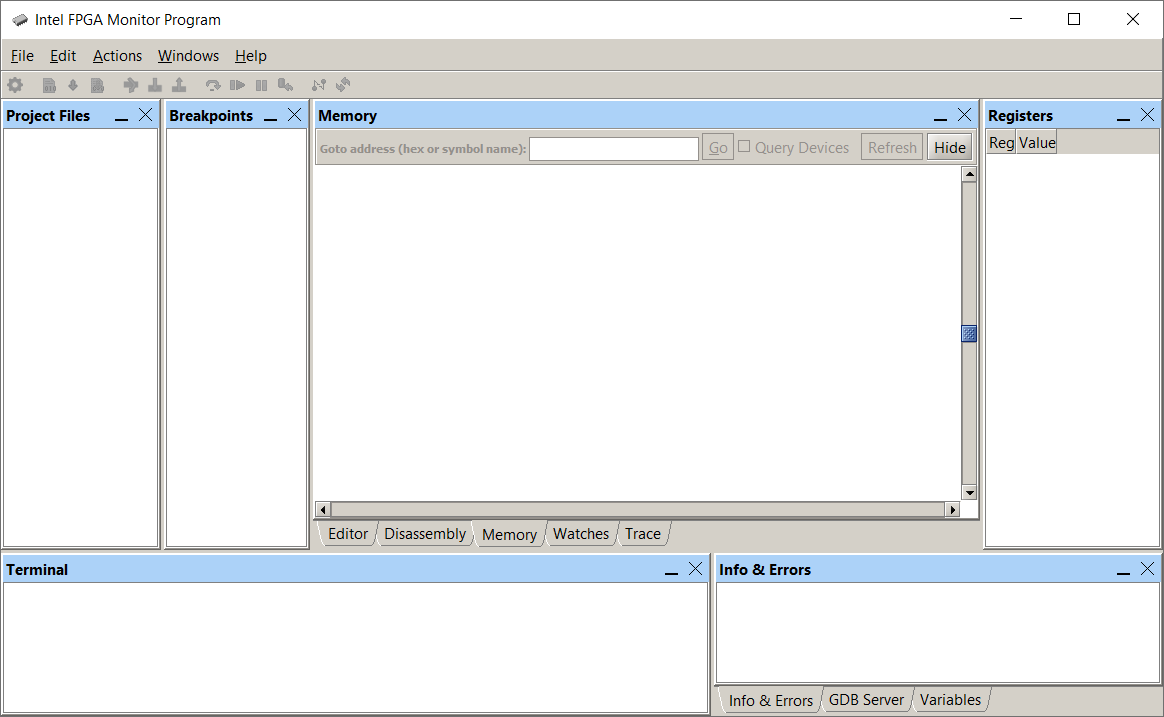
\includegraphics[scale=0.55]{screenshots/figure37.png}
   \end{center}
   \caption{The \productNameMed{} with a rearranged workspace.} 
	 \label{fig:37}
\end{figure}


\newpage
\section{Appendix A}

This appendix describes a number of Monitor Program features that
are useful for advanced debugging or other purposes.

\subsection{Using the Breakpoints Window}

In Section 3.6 we introduced instruction breakpoints and showed
how they can be set using the Disassembly window. Another way to
set breakpoints is to use the {\it Breakpoints} window, which is
depicted in Figure~\ref{fig:38}. This window supports three 
types of breakpoints in addition to the instruction breakpoint:
{\it read watchpoint}, {\it write watchpoint}, and 
{\it access watchpoint}, as follows:

\begin{itemize}
\item Read watchpoint - the processor is halted when a read
operation is performed on a specific address.
\item Write watchpoint - the processor is halted when a write
operation is performed on a specific address.
\item Access watchpoint - the processor is halted when a read or
write operation is performed on a specific address.
\end{itemize}


\begin{figure}[H]
   \begin{center}
      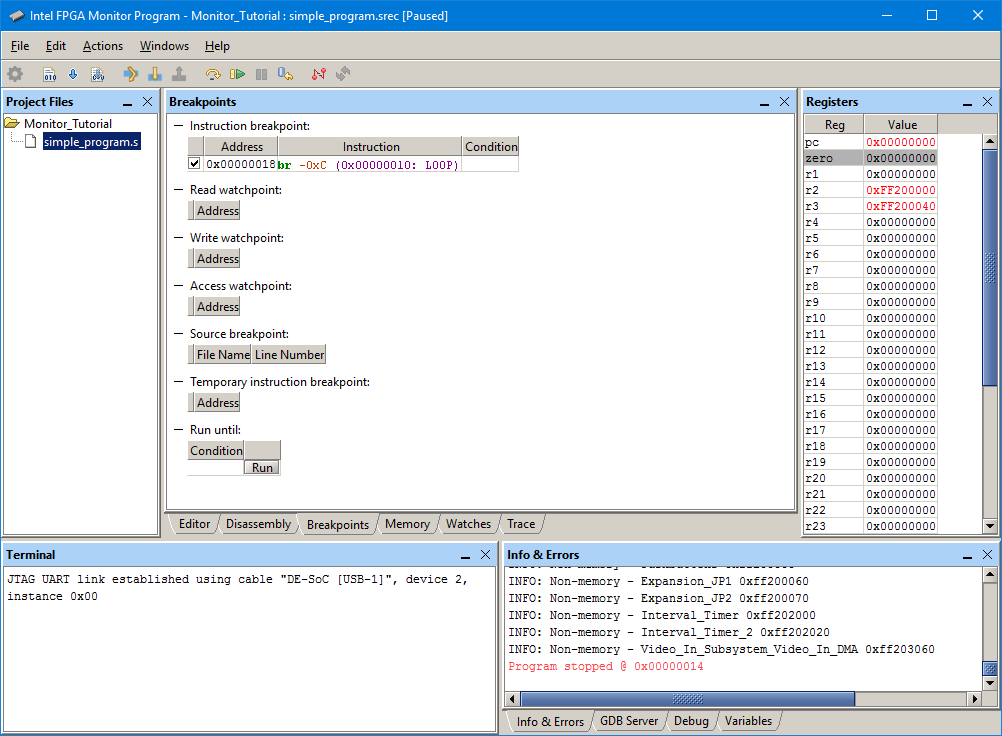
\includegraphics[scale=0.6]{screenshots/figure38.png}
   \end{center}
   \caption{The Breakpoints window.} 
	 \label{fig:38}
\end{figure}

In Figure~\ref{fig:38} an instruction breakpoint is shown for the 
address \texttt{0x00000018}. This corresponds to an address in
{\it simple\_program.s}. 
In Section 3.6 we showed how to create such an instruction
breakpoint by using the Disassembly window. But we could
alternatively have created this breakpoint by right-clicking in
a grey box under the label {\sf Instruction breakpoint} in 
Figure~\ref{fig:38} and then selecting {\sf Add}. A breakpoint can be
deleted by unchecking the box beside its address.

Setting a read, write, or access watchpoint is done by
right-clicking on the appropriate box in Figure~\ref{fig:38} and specifying
the desired address.

The Monitor Program also supports a type of breakpoint called a
{\it conditional breakpoint}, which triggers only when a 
user-specified condition is met. This type of breakpoint is
specified by double-clicking in the empty box {\it under} the 
label {\sf Condition} in Figure~\ref{fig:38} to open the dialog shown in 
Figure~\ref{fig:39}. The condition can be associated with an instruction
breakpoint, or it can be a stand-alone condition if entered in
the {\sf Run until} box in the Breakpoints window. 
As an example, we compiled and loaded the {\it simple\_program}
project. Then, we entered the condition \texttt{r4 == 5}. The
condition causes the breakpoint to trigger only if register
r4 contains the value 5. Thus, running this program causes the 
LEDs to display the current state of the slider switches as these
switches are set to different patterns. But, when the selected
pattern is 0x005, the conditional breakpoint will stop the
execution of the program.

Note that if a stand-alone condition is entered in the
{\sf Run until} box, then the Run button associated with this box must be used to run the
program, rather than the normal {\sf Actions > Continue} command.  
The processor runs much more slowly than in its normal execution
mode when a conditional breakpoint is being used.

\begin{figure}[H]
   \begin{center}
      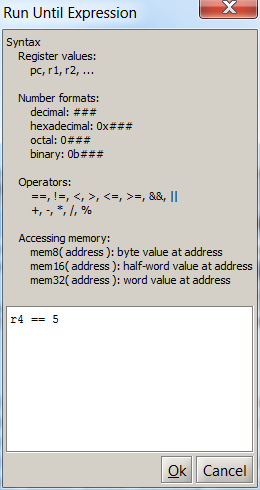
\includegraphics[scale=0.8]{screenshots/figure39.png}
   \end{center}
   \caption{The Conditional Breakpoint dialog.} 
	 \label{fig:39}
\end{figure}


\subsection{Working with the Memory Window}

The Memory window was shown in Figure~\ref{fig:20}. This window is
configurable in a variety of ways:

\begin{itemize}
\item Memory element size - the display can format the memory
contents as bytes, half-words (2-bytes), or words (4-bytes).
This setting can be configured by right-clicking on the Memory
window, as illustrated in Figure~\ref{fig:34}.

\begin{figure}[H]
   \begin{center}
      \includegraphics[scale=1]{screenshots/figure40.png}
   \end{center}
   \caption{Setting the memory element size.} 
	 \label{fig:40}
\end{figure}

\item Number of words per line - the number of words per line can
be configured to make it easier to find memory addresses, as
depicted in Figure~\ref{fig:41}.

\begin{figure}[H]
   \begin{center}
      \includegraphics[scale=1]{screenshots/figure41.png}
   \end{center}
   \caption{Setting the number of words per line.} 
	 \label{fig:41}
\end{figure}

\item Number format - this is similar to the number format option in the Register window described in Section 3.7,
and can be configured by right-clicking on the Memory window.

\item Display order - the Memory window can display addresses
increasing from left-to-right or right-to-left. 
\end{itemize}

\subsubsection{Character Display}

The \textsf{Memory} window can also be configured to interpret
memory byte values as ASCII characters. 
This is useful if one wishes to examine character strings that 
are stored in the memory.
For this purpose it is convenient to view
the memory in bytes and characters simultaneously so that the
characters appear in the correct sequence. This can be
accomplished by clicking the {\sf Switch to character mode} menu
item, as illustrated in Figure~\ref{fig:42}. A sample display in the
character mode is shown in Figure~\ref{fig:43}.
  
\begin{figure}[H]
   \begin{center}
      \includegraphics[scale=1]{screenshots/figure42.png}
   \end{center}
   \caption{Switching to the character mode.}
	 \label{fig:42}
\end{figure}

\begin{figure}[H]
   \begin{center}
      \includegraphics[scale=0.7]{screenshots/figure43.png}
   \end{center}
   \caption{Character mode display.}
	 \label{fig:43}
\end{figure}

It is possible to return to the previous memory view mode by
right-clicking and selecting the {\sf Revert to previous mode}
menu item.


\subsubsection{Memory Fill}

Memory fills can be performed in the Memory window. Click the
{\sf Actions > Memory fill} menu item or right-click on the
Memory window and select {\sf Memory fill}. 
A {\sf Memory fill} panel will appear on the left side of the
Memory window. Simply fill in the desired values and 
click {\bf Fill}. 

\subsubsection{Load File Data into Memory}

Data stored in a file can be loaded into the memory by using the
Memory window. This feature is accessed by selecting the command
{\sf Actions > Load file into memory} or by right-clicking on the
Memory window. The {\sf Load file} panel will appear on the left
side of the Memory window, as illustrated in Figure~\ref{fig:44}, to allow
the user to browse and select a data file.  The user provides a base address in memory where the data should be stored. 

\begin{figure}[H]
   \begin{center}
      \includegraphics[scale=0.6]{screenshots/figure44.png}
   \end{center}
   \caption{The Load file panel.}
	 \label{fig:44}
\end{figure}

The format of these files is illustrated in Figure~\ref{fig:45}. 
The file consists of any number of lines, where each line
comprises a comma-separated list of data values. Each data value
is expressed as a hexadecimal number with an optional $-$ sign.
Two additional parameters can be specified: the value of the
delimiter character (comma is the default), and size in bytes of
each data value (1 is the default).

\begin{figure}[H]
   \begin{center}
      \includegraphics[scale=0.7]{screenshots/figure45.png}
   \end{center}
   \caption{A Delimited hexadecimal value file.}
	 \label{fig:45}
\end{figure}

\subsection{Setting a Watch Expression}

Watch expressions provide a convenient means of keeping track of
the value of multiple expressions of interest. These expressions
are re-evaluated each time program execution is stopped. 
To add a watch expression:

\begin{enumerate}
\item Switch to the {\it Watches} window.

\item Right-click on the gray bar and click \textsf{Add},
as illustrated in Figure~\ref{fig:46}.

\begin{figure}[H]
   \begin{center}
      \includegraphics[scale=0.6]{screenshots/figure46.png}
   \end{center}
   \caption{The Watches window.}
	 \label{fig:46}
\end{figure}

\item The {\it Edit Watch Expression} window will appear, as
shown in Figure~\ref{fig:47}. The desired watch expression can then be
entered, using the syntax indicated in the window. In the figure,
the expression \texttt{mem32(sp)} is entered, which will display
the value of the data word at the current stack pointer address.

\begin{figure}[H]
   \begin{center}
      \includegraphics[scale=0.6]{screenshots/figure47.png}
   \end{center}
   \caption{The Edit Watch Expression window.}
	 \label{fig:47}
\end{figure}

\item Click \textsf{Ok}. The watch expression and its current
value will appear in the table. The number format of a value
displayed in the watch expression window can be changed by
right-clicking on the row for that value.  
As the program being debugged is repeatedly run, 
the watch expression will be re-evaluated each time and its value
will be shown in the table of watch values.
\end{enumerate}

\subsection{The GDB Server Panel (Advanced)}
To see this panel, select the {\sf GDB Server} panel of the
Monitor Program. This window will display the low-level commands
being sent to the GDB Server, used to interact with the HPS
system on the DE1-SoC board. It will also show the responses that GDB sends back. The Monitor Program provides the option
of typing GDB commands and sending them to the debugger. 
Consult online resources for the GDB program to learn what
commands are available.

\newpage
\section{Appendix B - Using Device Drivers (Advanced)}
Intel's development environment for Nios~II programs provides a
facility for using device driver functions for the I/O devices in
a hardware system. This facility, which is called the
{\it hardware abstraction layer} (HAL), is supported by the
Monitor Program. Using device driver functions is not recommended
for beginning students, and is intended for more advanced users. 

To see an example of code that uses device driver functions
create a project called {\it Monitor\_HAL}. 
Select the DE1-SoC Computer system. Set the program type to 
{\sf Program with Device Driver Support}, 
check {\sf Include a sample program with the project}, 
and select the sample program named {\it Media}. The source file
for this sample program is called {\it media.c}.
When creating this project, the New Project Wizard does not
display the screen for choosing memory settings, such as the one in Figure~\ref{fig:32}. This is because the HAL automatically chooses 
the necessary memory settings for projects that make use of device drivers.

The {\it media.c} program communicates with I/O devices by making
calls to device driver functions, rather than using memory-mapped
I/O as has been done in previous examples in this tutorial.  
To see some examples of such function-calls, examine the source
code in the file {\it media.c}. It calls device driver functions
for the audio devices in the DE1-SoC Computer, the VGA output
port, the PS/2 port, and parallel ports. The device driver
functions for each of these devices are defined in 
{\it include files} that are specified at the top of the
{\it media.c} file. The set of device driver functions
provided for an IP core is specified as part of the documentation
for that IP core.

Compile and load the program by using the command 
{\sf Actions > Compile \& Load}. 
The Monitor Program automatically compiles both the {\it media.c}
program and all device drivers that it uses. In subsequent
compilations of the program, only the {\it media.c} code is
compiled. 

Run the program. It performs the following: 
\begin{itemize}
\item
Records audio for about 10 seconds when KEY[1] is pressed. 
LEDR[0] is lit while recording.
\item 
Plays the recorded audio when KEY[2] is pressed. LEDR[1] is lit while playing.
\item
Draws a blue box on the VGA display, and places a text string inside the box.
\item
Shows on the HEX displays the last three bytes of data received from a device connected to the PS/2 port. 
\end{itemize}

More details about developing programs with the Monitor Program
that use HAL device drivers can be found in the tutorial 
{\it Using HAL Device Drivers with the \productNameMed{}}, which is available in the University Program section of Intel's
website. More information about HAL can be found in the
{\it Nios~II Software Developer's Handbook}.


%%%%%%%%%%%%%%%%%%%%%%%%%%%%%%%%%%%
%%% Running Multiple Instances of the Monitor Program (Advanced)
\newpage
\section{Appendix C - Running Multiple Instances of the Monitor Program (Advanced)}

In some cases it may be useful to run more than one instance of
the Monitor Program on the same computer. For example, the
selected system may contain more than one processor. 
An instance of the Monitor Program is required to run and debug
programs on each available processor. As described in 
Section 3.1, it is possible to select a particular processor
in a system via the \textsf{Processor} drop-down
list in the {\it New Project Wizard} and {\it Project Settings}
windows.

The Monitor Program uses the {\it GDB Server} to interact with
the HPS system, and connects to the GDB Server using TCP ports.
By default, the Monitor Program uses port 2399 as the base port,
and to connect to each processor in a system the Monitor Program
will attempt to use a port located at a fixed offset from this
base port. For example, a single system consisting of four
processors corresponds to ports 2399-2402.

However, the Monitor Program does not detect any ports that may
already be in use by other applications. If the Monitor Program
fails to connect to the GDB Server due to a port conflict, then
the base port number can be changed by creating an environment
variable called \texttt{ALTERA\_MONITOR\_DEBUGGER\_BASE\_PORT}
and specifying a different number.

It is also possible to have more than one board connected to
the host computer. As described in Section 3.1, a particular
board can be selected via the \textsf{Host connection} drop-down
list in the {\it New Project Wizard} and {\it Project Settings}
windows. In this case, a separate instance of the Monitor
Program is needed to interact with each processor on each
physical board. By default, the Monitor Program assumes a
maximum of ten Nios~II processors per board. This means that
ports 2399-2408 are used by the Monitor Program for the first
board connected to the computer, and the first processor on the
second board will use port 2409.

It is possible to specify a different value for the maximum
number of processors per Nios~II hardware system by creating an
environment variable called 
\texttt{ALTERA\_MONITOR\_DEBUGGER\_MAX\_PORTS\_PER\_CABLE} and
specifying a different number. 
This is useful if a system contains more than ten Nios~II
processors. It is also useful if a port conflict exists and none
of the systems contain ten or more processors. In this case,
decreasing this number (in conjunction with changing the base
port number) may provide a solution.


%%%%%%%%%%%%%%%%%%%%%%%%%%%%%%%%%%%
%%% Examining the Instruction Trace
\newpage
\section{Appendix D - Examining the Instruction Trace (Advanced)}

An instruction trace is a hardware-level mechanism to record a
log of all recently executed instructions. 
The \emph{Nios~II JTAG Debug Module} has the instruction trace
capability, but only if a Level 3 or higher debugging level
is selected in the \emph{SOPC Builder} or \emph{Platform Designer}
configuration of the JTAG Debug Module 
(See the \emph{Nios~II Processor Reference Handbook},
available from Intel, for more information about the
configuration settings of the JTAG Debug Module). If the 
required JTAG Debug Module is not present, a message will be
shown in the \textsf{Info \& Errors} window of the Monitor
Program after loading a program, to indicate that instruction
trace is not available.

The {\it Trace} feature is disabled by default. To enable 
the trace feature, go to the Trace window, right click inside
the window, then select \textsf{Enable Trace}. To view the 
instruction trace of a program, go to the Trace window
after pausing the program during execution. As shown in 
Figure~\ref{fig:48}, the instructions are grouped into
different colored blocks and labeled alphabetically. 
The number of times each instruction block is executed is
shown beneath its alphabetical label.

\begin{figure}[H]
   \begin{center}
      \includegraphics[scale=0.5]{screenshots/figure48.png}
   \end{center}
   \caption{The Trace window.}
	 \label{fig:48}
\end{figure}

Right-clicking anywhere in the Trace window brings up
several options, as shown in Figure~\ref{fig:49}.
The Trace feature can be turned on or off by selecting
the \textsf{Enable trace} or \textsf{Disable trace} options. 
It is also possible to toggle the {\it debug events} in the 
trace on or off by selecting \textsf{Show debug events}, or
clear current trace sequences by selecting 
\textsf{Clear trace sequences}. 

\begin{figure}[H]
   \begin{center}
      \includegraphics[scale=0.5]{screenshots/figure49.png}
   \end{center}
   \caption{Right-click options in the Trace window.}
	 \label{fig:49}
\end{figure}

Running the program using the \textsf{Actions > Continue} or
\textsf{Actions > Single Step} commands will show up in the
trace sequence as {\it debug events} after each time the
program pauses execution, as shown in 
Figure~\ref{fig:50}.

\begin{figure}[H]
   \begin{center}
      \includegraphics[scale=0.5]{screenshots/figure50.png}
   \end{center}
   \caption{The Trace window with various debug events.}
	 \label{fig:50}
\end{figure}

If the {\it pc} value is changed before the program continues 
to run, the Monitor Program will insert a gap sequence in the
trace, as shown in Figure~\ref{fig:51}. 
The \textsf{Actions > Restart} command will set the {\it pc}
value back to the initial starting address. The {\it pc} 
value can also be arbitrarily set by double clicking its value 
in the \textsf{Registers} window and editing
its hexadecimal value. 

\begin{figure}[H]
   \begin{center}
      \includegraphics[scale=0.5]{screenshots/figure51.png}
   \end{center}
   \caption{A gap sequence in the instruction trace.}
	 \label{fig:51}
%   \label{fig:trace_4}
\end{figure}

Breakpoints in the program will also show up in the trace
sequence as a {\it debug event} each time the breakpoint
condition is met, as illustrated in Figure~\ref{fig:52}.

\begin{figure}[H]
   \begin{center}
      \includegraphics[scale=0.5]{screenshots/figure52.png}
   \end{center}
   \caption{A breakpoint in the instruction trace.}
	 \label{fig:52}
\end{figure} 

\subsubsection{Note About Tracing Interrupt Sequences}
It is possible that interrupt sequences are happening in the
program, yet do not show up in the Trace window in 
the Monitor Program. This is because the instruction blocks
shown in the trace sequence are actually sampled from a window 
of time over the entire program execution. As a result, the
interrupt sequences may not be included in the sample of
instruction blocks displayed in the Monitor Program. 
One way to deal with this problem is to trigger a breakpoint
after an interrupt finishes executing.

\section{Appendix D - Configuration File}
The Monitor Program configuration file allows default values to be set for project creation. The monitor program searches 
{\sf \$(UniversityProgramRoot)/amp.config} for the configuration file, where {\sf UniversityProgramRoot} is the path to the 
University Program directory in the Quartus installation.\\
For example {\sf C:/intelFPGA/16.1/University\_Program/amp.config}.

To change the default path to the configuration file, add the following command line argument 
when running the Monitor Program: {\sf \texttt{-}\texttt{-}config-file=<Path to File>}

Table~\ref{tbl:2} summarizes the configuration options available in the Monitor Program.

\begin{table}[h]
    \centering
    \begin{tabular}{|l|p{5in}|}
        \hline
        Flag & Explanation\\
        \hline\hline
				\hline
				project\_name				& The project name.\\
				project\_path				& The new project directory path.\\
				architecture				& The architecture.\\
				system							& The default sample system to be used (ex. DE1-SoC Computer)\\
				c\_compiler\_flags	& C Compiler flags\\
				c\_linker\_flags		& C Linker flags\\
				use\_small\_c\_lib	& Boolean to use the small C Library (Nios II)\\
				emulate\_instr			& Boolean to emulate unimplemented instructions\\
				include\_system\_info\_file & Boolean whether to include the system info header by default.\\
				answer\_for\_reload\_file & {\it yes} or {\it no} option to bypass the file reload dialog when files are edited outside the program. If undefined, the dialog will be shown.\\
				\hline
    \end{tabular}
    \caption{Configuration Flags and Default Options.} 
		\label{tbl:2}
\end{table}

The configuration file uses white space or an equal sign as a delimiter, for example: 
{\sf flag	option} or {\sf flag=option}. Where {\it flag} is one of the values in the first column of 
Table~\ref{tbl:2} and {\it option} is the default value for that flag. Number signs 
(\#) can be used to add comments to the configuration file. Lines starting with the symbol will
not be processed with the configuration file. Boolean values can use integers or case insensitive strings. 
Options of 'false', 'no' and '0' will all produce a false Boolean, any other values will produce a true Boolean.

% Copyright and Trademark

%\newcommand{\datePublished}{Mar 2022}

\newcommand{\versnum}{21.1} %version number quartus/AMP
\newcommand{\quartusname}{Quartus\textsuperscript{\textregistered} Prime}	
\newcommand{\textBar}{For \quartusname{} \versnum{}}
\newcommand{\thisyear}{2022 } %for copyright
\newcommand{\company}{FPGAcademy.org}
\newcommand{\longteamname}{FPGAcademy.org}
\newcommand{\teamname}{FPGAcademy}
\newcommand{\website}{FPGAcademy.org}

\newcommand{\productAcronym}{AMP}
\newcommand{\productNameShort}{Monitor Program}

\newcommand{\productNameMedTM}{Monitor Program}
\newcommand{\productNameMed}{Monitor Program}

%\newcommand{\headerLogoFilePath}[1]{#1/FPGAcademy.png}



%%%%%%%%%%%%%%%%%%%%%%%%%%%%%%%%%%%%%%%%
%%% FPGAcademy Copyright Information %%%
%%%%%%%%%%%%%%%%%%%%%%%%%%%%%%%%%%%%%%%%

%Always put the copyright on a new page (clear page), with some vertical space from top
\clearpage
\vspace{1in}

\noindent

Copyright {\copyright} FPGAcademy.org. All rights reserved. FPGAcademy and the FPGAcademy logo are trademarks of  FPGAcademy.org.  This document is being provided on an ``as-is'' basis and as an accommodation and therefore all warranties, representations or guarantees of any kind (whether express, implied or statutory) including, without limitation, warranties of merchantability, non-infringement, or fitness for a particular purpose, are specifically disclaimed.

%FPGAcademy assumes no responsibility or liability arising out of the application or use of any information,  product,  or  service  described  herein  except  as  expressly  agreed  to  in  writing  by  FPGAcademy.



**Other names and brands may be claimed as the property of others.




\end{document}
